\documentclass[a4paper,12pt,twoside,openany]{report}
%
% Wzorzec pracy dyplomowej
% J. Starzynski (jstar@iem.pw.edu.pl) na podstawie pracy dyplomowej
% mgr. Błażeja Wincenciaka
% Wersja 3.0 - 10 stycznia 2009
%
\usepackage{polski}
\usepackage[utf8]{inputenc}
\usepackage[pdftex]{graphicx}
\usepackage{tabularx}
\usepackage{array}
\usepackage[polish]{babel}
\usepackage{subfigure}
\usepackage{amsfonts}
\usepackage{verbatim}
\usepackage{indentfirst}
\usepackage[pdftex]{hyperref}

% dodatkowe paczki
\usepackage{mathtools}
\usepackage{textcomp}
\usepackage{siunitx}


% rozmaite polecenia pomocnicze
% gdzie rysunki?
\newcommand{\ImgPath}{.}

% oznaczenie rzeczy do zrobienia/poprawienia
\newcommand{\TODO}{\textbf{TODO}}


% wyroznienie slow kluczowych
\newcommand{\tech}{\texttt}

% na oprawe (1.0cm - 0.7cm)*2 = 0.6cm
% na oprawe (1.1cm - 0.7cm)*2 = 0.8cm
%  oddsidemargin lewy margines na nieparzystych stronach
% evensidemargin lewy margines na parzystych stronach
\def\oprawa{1.05cm}
\addtolength{\oddsidemargin}{\oprawa}
\addtolength{\evensidemargin}{-\oprawa}

% table span multirows
\usepackage{multirow}
\usepackage{enumitem}	% enumitem.pdf
\setlist{listparindent=\parindent, parsep=\parskip} % potrzebuje enumitem

%%%%%%%%%%%%%%% Dodatkowe Pakiety %%%%%%%%%%%%%%%%%
\usepackage{prmag}   % definiuje komendy opieku,nrindeksu, rodzaj pracy, ...



%%%%%%%%%%%%%%% Strona Tytułowa %%%%%%%%%%%%%%%%%
% To trzeba wypelnic swoimi danymi
\title{Dwukołowy robot inspekcyjny}

% autor(zy)
\author{Mateusz Staszków}
\nrindeksu{261006}
% wstawienie zdjecia
\zdjecie{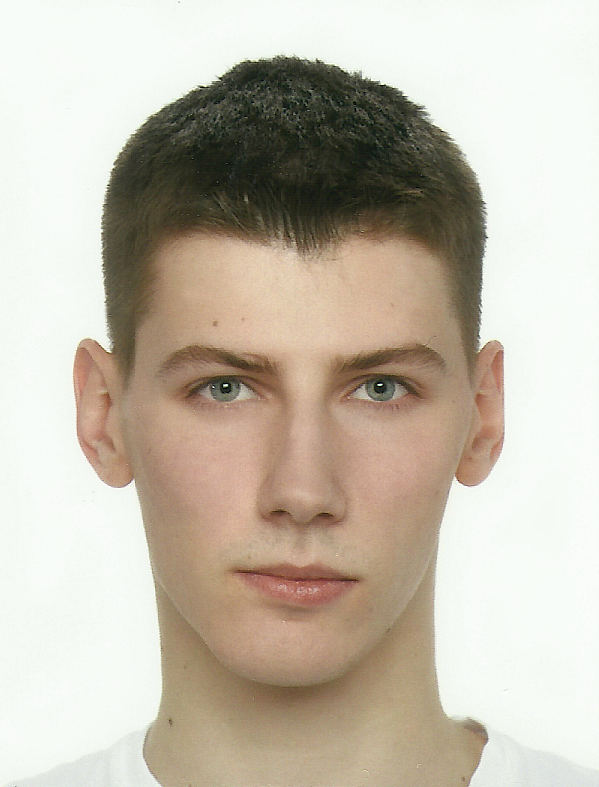
\includegraphics[width=4cm]{\ImgPath/zdjecie-kor.png}}

\opiekun{dr inż. Krzysztof Bieńkowski}
% opcjonalnie: \konsultant{prof. Dzielny Konsultant}
\terminwykonania{31 maja 2017} % data złożenia - pokazana na stronie tytułowej
\datawydaniatematu{1 października 2016}
\rokakademicki{2016/2017}

% zakres pracy
\zakres{\begin{enumerate}
 \item Przegląd istniejących rozwiązań
 \item Projekty układu
 \item Budowa robota
 \item Implementacja programów sterujących
 \item Testy i analiza
\end{enumerate}}


% Podziekowanie - opcjonalne
\podziekowania{\noindent
{\Large Podziękowania}
\bigskip

Dziękuję bardzo serdecznie Rodzinie, Wykładowcom, Władzom Politechniki i Promotorowi - dr inż. Krzysztofowi Bieńkowskiemu

\bigskip

{\raggedleft
Mateusz Staszków

}

}

% To sa domyslne wartosci
% - mozna je zmienic, jesli praca jest pisana gdzie indziej niz w ZETiIS
% - mozna je wyrzucic jesli praca jest pisana w ZETiIS
\miasto{Warszawa}
\uczelnia{POLITECHNIKA WARSZAWSKA}
\wydzial{WYDZIAŁ ELEKTRYCZNY}
\instytut{INSTYTUT STEROWANIA \linebreak[1] I~ELEKTRONIKI PRZEMYSŁOWEJ}
\zaklad{ZAKŁAD MASZYN ELEKTRYCZNYCH}
\rodzajpracy{INŻYNIERSKA}
\kierunekstudiow{AUTOMATYKA I ROBOTYKA}
%%% koniec od P.W

\opinie{%
  %\newpage
\begin{center}
 {\large\bf  Opinia} \\
o pracy dyplomowej magisterskiej wykonanej przez dyplomanta\\
{\bf Zdolnego Studenta i Pracowitego Kolegę} \\
 Wydział Elektryczny, kierunek Informatyka,  Politechnika Warszawska\\
Temat pracy\\
\textit{\bf
TYTUŁ PRACY DYPLOMOWEJ
}\\
\end{center}
\medskip
\noindent
Kierownik pracy dyplomowej: {\bf dr inż. Adam Niewymagający}\\
Ocena pracy dyplomowej: {\bf bardzo dobry}

\medskip

\centerline{\bf Treść opinii}
   Celem pracy dyplomowej panów dolnego Studenta i Pracowitego Kolegi  było
opracowanie systemu pozwalającego symulować  i opartego o oprogramowanie o
otwartych źródłach (ang. Open Source). Jak piszą Dyplomanci, starali się opracować
system, który łatwo będzie dostosować do zmieniających się dynamicznie wymagań,
będzie miał niewielkie wymagania sprzętowe i umożliwiał dalszą łatwą rozbudowę oraz
dostosowanie go do potrzeb.
Przedstawiona do recenzji praca składa się z krótkiego wstępu jasno i
wyczerpująco opisującego oraz uzasadniającego cel pracy, trzech rozdziałów (2-4)
zawierających opis istniejących podobnych
rozwiązań, komponentów rozpatrywanychjako kandydaci do
tworzonego systemu i wreszcie zagadnień wydajności wirtualnych
rozwiązań. Piąty rozdział to opis przygotowanego przez
Dyplomantów środowiska obejmujący opis konfiguracji
środowiska oraz przykładowe ćwiczenia laboratoryjne. Ostatni
rozdział pracy to opis możliwości dalszego
rozwoju projektu. W ramach przygotowania pracy Dyplomanci zebrali i przedstawili w
bardzo przejrzysty sposób duży zasób informacji, co świadczy o dobrej orientacji
w nowoczesnej i ciągle intensywnie rozwijanej tematyce stanowiącej
zakres pracy i o umiejętności przejrzystego przedstawienia tych
wyników. Praca zawiera dwa dodatki, z których pierwszy obejmuje wyniki
eksperymentów i badań nad wydajnością, a drugi to źródła
skryptów budujących środowisko.

 Dyplomanci dość
dobrze zrealizowali postawione przed nimi zadanie,
wykazali się więc umiejętnością zastosowania w praktyce wiedzy
przedstawionej w rozdziałach 2-4.  Uważam, że cele postawione w założeniach pracy zostały pomyślnie
zrealizowane. Proponuję ocenę bardzo dobrą (5).

\vskip 1cm
{
\raggedleft
(data, podpis)\kern1cm

}
  \newpage
  %\newpage
\begin{center}
 {\large\bf  Recenzja } \\
pracy dyplomowej magisterskiej wykonanej przez dyplomanta\\
{\bf Zdolnego Studenta i Pracowitego Kolegę} \\
 Wydział Elektryczny, kierunek Informatyka,  Politechnika Warszawska\\
Temat pracy\\
\textit{\bf
TYTUŁ PRACY DYPLOMOWEJ
}\\
\end{center}
\medskip
\noindent
Recenzent: {\bf prof. nzw. dr hab. inż. Jan Surowy}\\
Ocena pracy dyplomowej: {\bf bardzo dobry}
\medskip


\centerline{\bf Treść recenzji}
   Celem pracy dyplomowej panów dolnego Studenta i Pracowitego Kolegi  było
opracowanie systemu pozwalającego symulować  i opartego o oprogramowanie o
otwartych źródłach (ang. Open Source). Jak piszą Dyplomanci, starali się opracować
system, który łatwo będzie dostosować do zmieniających się dynamicznie wymagań,
będzie miał niewielkie wymagania sprzętowe i umożliwiał dalszą łatwą rozbudowę oraz
dostosowanie go do potrzeb.
Przedstawiona do recenzji praca składa się z krótkiego wstępu jasno i
wyczerpująco opisującego oraz uzasadniającego cel pracy, trzech rozdziałów (2-4)
zawierających bardzo solidny i przejrzysty opis: istniejących podobnych
rozwiązań (rozdz. 2), komponentów rozpatrywanychjako kandydaci do
tworzonego systemu (rozdz. 3) i wreszcie zagadnień wydajności wirtualnych
rozwiązań, zwłaszcza w kontekście współpracy  kilku elementów
 sieci (rozdział 4). Piąty rozdział to opis przygotowanego przez
Dyplomantów środowiska obejmujący opis konfiguracji
środowiska oraz przykładowe ćwiczenia laboratoryjne (5 ćwiczeń). Ostatni, szósty
rozdział pracy to krótkie zakończenie, które wylicza także możliwości dalszego
rozwoju projektu. W ramach przygotowania pracy Dyplomanci zebrali i przedstawili w
bardzo przejrzysty sposób duży zasób informacji o narzędziach, Rozdziały 2, 3 i 4 świadczą o dobrej orientacji
w nowoczesnej i ciągle intensywnie rozwijanej tematyce stanowiącej
zakres pracy i o umiejętności syntetycznego, przejrzystego przedstawienia tych
wyników. Drobne  mankamenty tej części pracy to zbyt skrótowe omawianie
niektórych zagadnień technicznych, zakładające dużą początkową wiedzę czytelnika
i dość niestaranne podejście do powołań na źródła.
Utrudnia to w pewnym stopniu czytanie pracy i zmniejsza jej wartość dydaktyczną
(a ta zdaje się być jednym z celów Autorów), ale jest zrekompensowane zawartością
merytoryczną. Praca zawiera dwa dodatki, z których pierwszy obejmuje wyniki
eksperymentów i badań nad wydajnością, a drugi to źródła
skryptów budujących środowisko. Praca
zawiera niestety dość dużą liczbę drobnych błędów redakcyjnych, ale nie wpływają
one w sposób istotny na na jej czytelność i wartość. W całej pracy przewijają
się samodzielne, zdecydowane wnioski Autorów, które są wynikiem własnych i
oryginalnych badań.  Rozdział 5 i dodatki pracy przekonują mnie, że Dyplomanci dość
dobrze zrealizowali postawione przed nimi zadanie. Pozwala to stwierdzić, że
wykazali się więc także umiejętnością zastosowania w praktyce wiedzy
przedstawionej w rozdziałach 2-4. Kończący pracę rozdział szósty świadczy o
dużym (ale moim zdaniem uzasadnionym) poczuciu własnej wartości i jest
świadectwem własnego, oryginalnego spojrzenia na tematykę przedstawioną w pracy
dyplomowej. Uważam, że cele postawione w założeniach pracy zostały pomyślnie
zrealizowane. Proponuję ocenę bardzo dobrą (5).

\vskip 1cm
{
\raggedleft
(data, podpis)\kern1cm

}
}


\begin{document}
\maketitle

%-----------------
% Wstęp
%-----------------
\chapter{Wstęp}

Roboty inspekcyjne znajdują zastosowanie najczęściej w miejscach trudno dostępnych dla człowieka. Można również spotkać małe roboty przeszukujące korytarze w biurowcach w godzinach nocnych. Ich zadaniem jest odwiedzenie lub zeskanowanie każdego miejsca w budynku i upewnienie się czy wszystko jest zachowane w ustalonym porządku.

Problem stabilizacji położenia w pionie dotyczy wielu gałęzi przemysłu, na przykład takich jak: produkcja jednoosobowych transportowych pojazdów typu Segway na lotniskach i w centrach handlowych, układy balansujące na nierównych powierzchniach, czy nawet roboty humanoidalne.

Połączenie tych dwóch cech czyni robota pomocnym w trudno dostępnych miejscach zarówno jeżeli chodzi o toksyczność jak i bardzo nieregularną powierzchnię jezdną.

Dwukołowy robot balansujący działa na zasadzie wahadła odwróconego. Jego zadaniem jest ciągłe utrzymywanie pionu z możliwie jak najmniejszymi odchyłami. Jest to układ niestabilny i wymaga automatycznej regulacji - zadanie to spełnia regulator liniowo-kwadratowy-Gaussa. \\
W układzie za sprzężenia zwrotne odpowiadają czujniki położenia, a dokładniej przyspieszenia - akcelerometr i prędkości kątowej - żyroskop. Do sterowania silnikami jest użyte sprzężenie zwrotne w postaci pomiaru położenia kół przez enkodery magnetyczne. Elektronika znajduje się na wytrawionych płytkach PCB. Układ jest zasilany z akumulatora litowo-polimerowego. Robot jest zaprojektowany tak, aby każdy element był jak najlżejszy i można było go łatwo wymienić. Stąd duża ilość śrub i mocowań na wcisk. Przy każdym mikrokontrolerze znajduje się złącze programatora, co umożliwia bezproblemowe aktualizowanie oprogramowania. Do komunikacji robota z otoczeniem służą czujniki ultradźwiękowe. Moduł WiFi umożliwia komunikację z komputerem PC i odczyt wszystkich pomiarów.

  %-----------------
  % Postawienie zadania
  %-----------------
\section{Postawienie zadania}

Zadaniem pracy jest przedstawienie konstrukcji autonomicznego i balansującego robota inspekcyjnego oraz przedstawienie działania za pośrednictwem wykresów i tabel.

Budowa robota to złożone zadanie i wymaga podzielenia na mniejsze elementy konstrukcji:
\begin{enumerate}
	\item Przeczytanie literatury na temat: 
    \begin{itemize}
    	\item balansujących i inspekcyjnych robotów komercyjnych, 
        \item dokumentacji technicznych mikrokontrolerów serii AVR i ARM, czujników ultradźwiękowych, akcelerometrów i żyroskopów, modułów WiFi, enkoderów, silników,
        \item dekodowania sygnałów z wyżej wymienionych czujników,
        \item szeregowej komunikacji przewodowej i bezprzewodowej,
        \item druku 3D,
        \item technologii wytwarzania płytek elektronicznych,
    \end{itemize}
	\item Zaprojektowanie:
    	\begin{itemize}
    		\item modelu matematycznego i modelu sterowania w środowisku Matlab i Simulink,
        	\item elektroniki w środowisku Cadsoft EAGLE,
        	\item modelu 3D w programie AutoCAD, podzielenie na części i wyeksportowanie do formatu, STL,
    	\end{itemize}
    \item Zakup elementów elektronicznych,
	\item Wydrukowanie części na drukarce 3D i sklejenie ich acetonem,
	\item Wytrawienie płytek PCB w nadsiarczanie sodu,
	\item Lutowanie elementów elektronicznych do płytek,
	\item Skonfigurowanie środowisk programistycznych,
    \item Wykonanie szkieletów kodu,
    \item Wzajemne skomunikowanie mikrokontrolerów,
    \item Oprogramowanie czujników,
    \item Implementacja:
    	\begin{itemize}
    		\item sterownika silników DC,
        	\item komunikacji mikrokontrolera z komputerem PC,
        	\item regulacji położenia w pionie (LQG),
            \item systemu skanowania pomieszczeń,
    	\end{itemize}
    \item Testy i analiza,
    \item Wnioski.
\end{enumerate}

%-----------------
% Mechanika
%-----------------
\chapter{Mechanika}
Robot został zaprojektowany tak, aby był jak najlżejszy. Ułatwia to sterowanie jego położeniem przy odpowiednio dobranych silnikach. Środek ciężkości znajduje się jak najwyżej, co przekłada się na ułatwienie sterowania położenia w pionie - układ gwałtowniej odpowiada na zadane wartości.

  %-----------------
  % Parametry ogólne
  %-----------------
\section{Parametry ogólne}

\noindent Masa: 1 kg\\
Wymiary: 95 mm x 180 mm x 306 mm\\
Wysokość środka masy: 162.6 mm\\
Moment bezwładności dla osi położonej w środku masy: 0.01 $kgm^2$\\

\begin{figure}[!htbp]
	\begin{center}
\centering
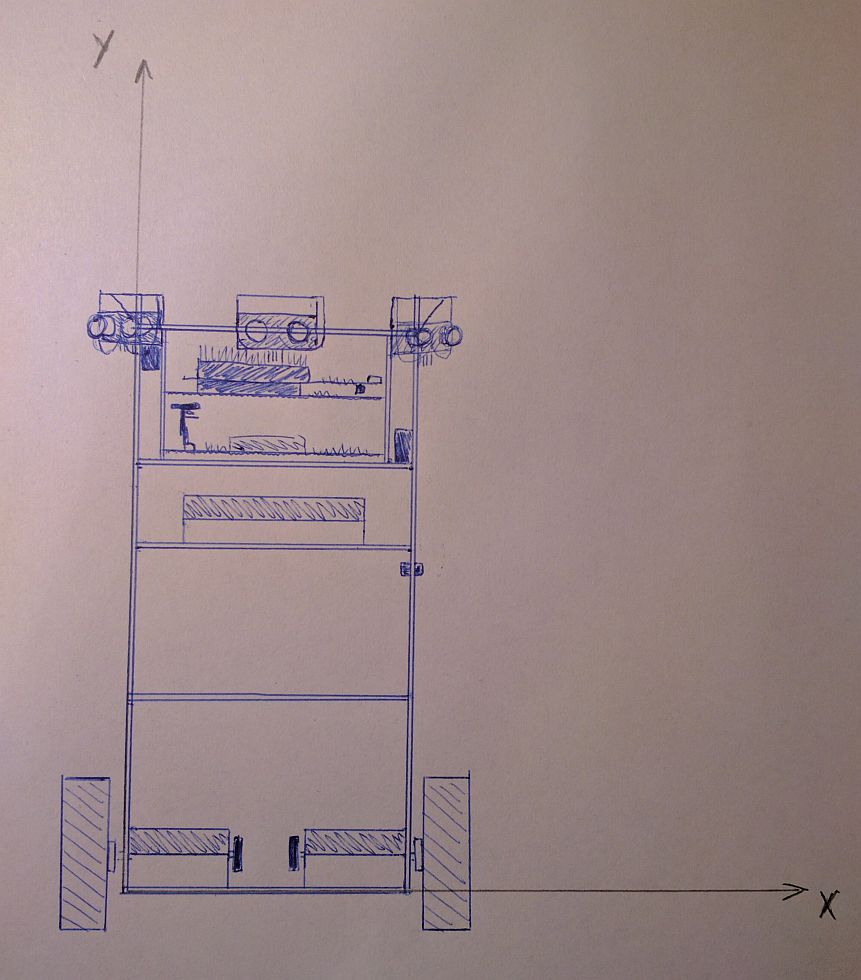
\includegraphics[scale=0.25]{\ImgPath/koncepcja.jpg}
\end{center}
	\caption{Koncepcja obudowy robota [opracowanie własne]}
	\label{model3d}
\end{figure}

\newpage
  %-----------------
  % Model 3D
  %-----------------
\section{Model 3D}
Model został zbudowany w programie Autodesk AutoCAD 2017. Następnie został podzielony na części w taki sposób, aby wydruk 3D był jak najmniej kłopotliwy. Każda część jest nie większa niż 100 mm x 180 mm x 80 mm. Następnie modele zostały wyeksportowane do formatu STL.

\begin{figure}[!htbp]
	\begin{center}
\centering
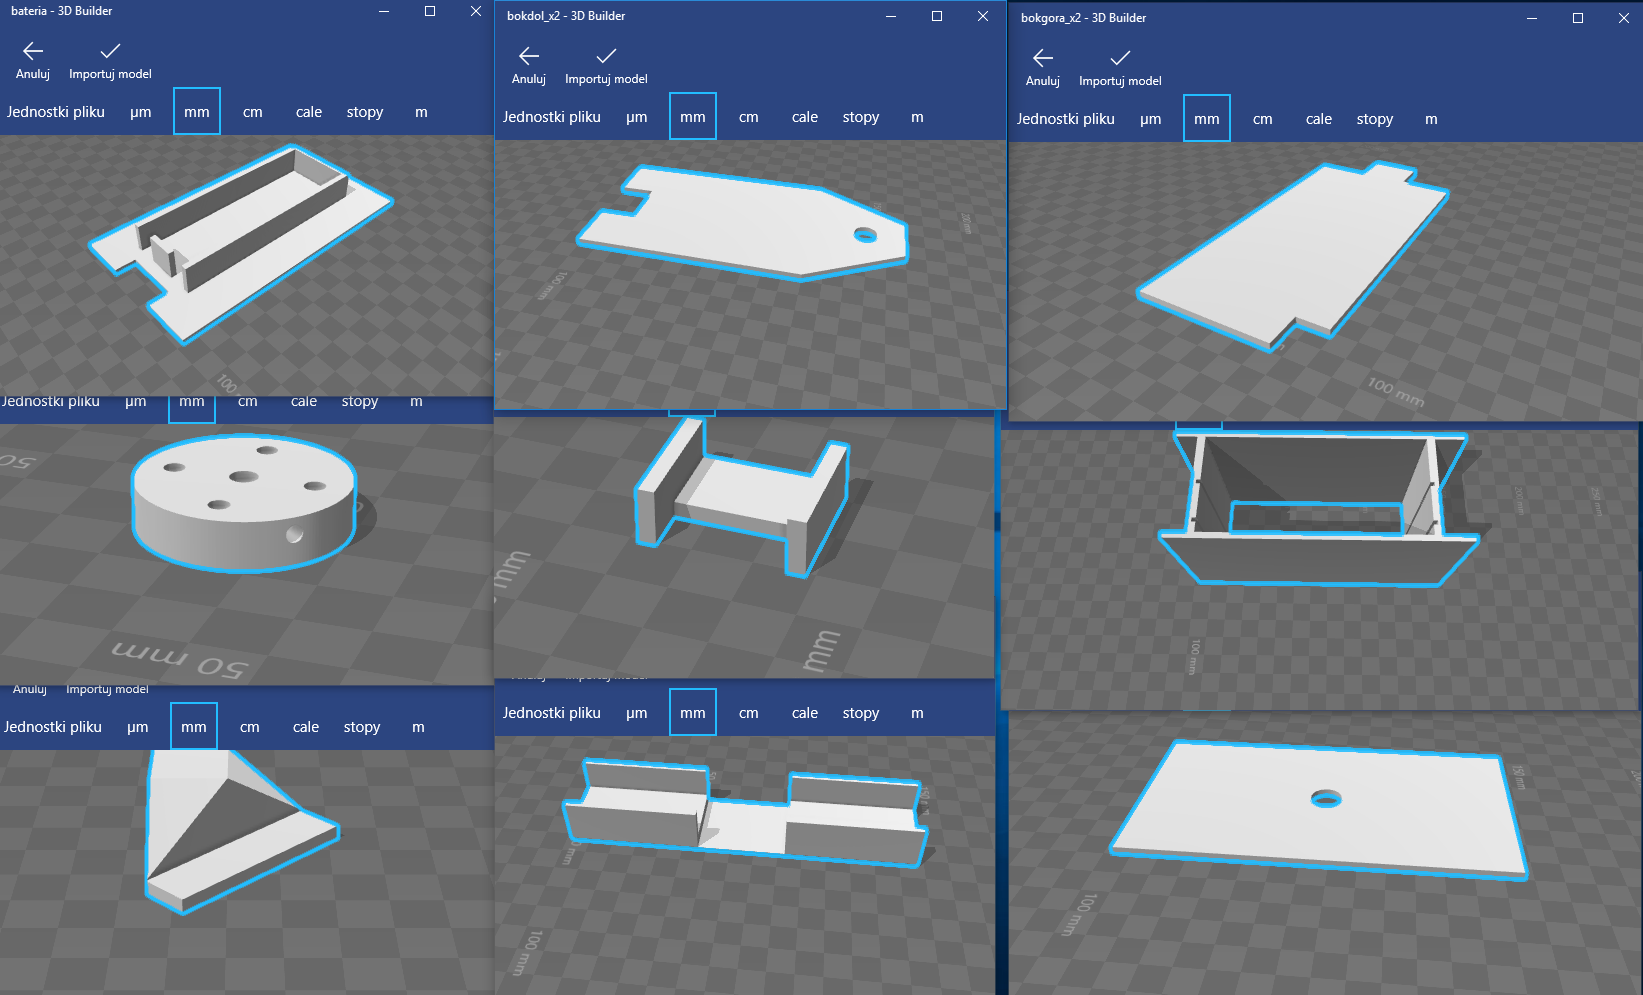
\includegraphics[scale=0.3]{\ImgPath/druki3d.PNG}
\end{center}
	\caption{Model 3D podzielony na części i wyeksportowany do STL [opracowanie własne]}
	\label{druki3d}
\end{figure}

  %-----------------
  % Obudowa
  %-----------------
\section{Obudowa}

\noindent Masa: 402 g\\
Wymiary: 95 mm x 180 mm x 306 mm\\

Obudowa została w całości wydrukowana na drukarce 3D, a poszczególne elementy są połączone acetonem. Proces adhezyjnego klejenia części jest możliwy poprzez użycie jako materiału do drukowania tworzywa ABS - kopolimeru akrylonitrylo-butadieno-styrenowego, który reagując z acetonem rozpuszcza się, umożliwiając, poprzez zbliżenie do niego innego materiału na przyklejenie się. 
\newpage
\noindent Obudowa składa się z czterech segmentów - kolejno od dołu:
\begin{itemize}
\item segment silników - odpowiadający za napęd robota, silniki są przykręcone do ścian bocznych za pomocą śrub i znajdują się w specjalnie zaprojektowanych miejscach, aby ograniczyć ich ruch. Takie zamontowanie umożliwia ich łatwą i szybką wymianę. W ścianach bocznych umieszczono łożyska, w których znajdują się wały silników,
\item część akumulatora - odpowiadająca za zasilanie, akumulator ma swój koszyk, co umożliwia łatwą wymianę i odpowiednie usztywnienie pakietu ogniw,
\item część elektroniczna: sciany z otworami na wciśnięcie płytki PCB i z koszykiem na żyroskop/akcelerometr na spodzie najwyższej półki,
\item część komunikacyjna: znajdują się tu miejsca na 3 czujniki ultradźwiękowe oraz na moduł Wi-Fi.
\end{itemize}

\begin{figure}[!htbp]
	\begin{center}
\centering
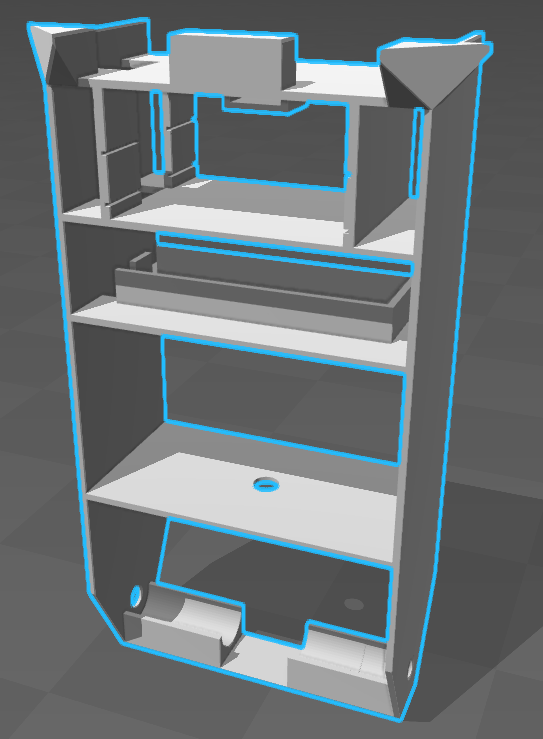
\includegraphics[scale=0.4]{\ImgPath/model3d.PNG}
\end{center}
	\caption{Cała obudowa zaprojektowana w programie Autodesk AutoCAD i wyeksportowana do pliku STL [opracowanie własne]}
	\label{model3d}
\end{figure}

\newpage

  %-----------------
  % Napęd
  %-----------------
\section{Napęd}

Do napędu robota zostały użyte silniki prądu stałego firmy Pololu na napięcie 12 V z przekładnią 9.68 : 1 (25Dx48L) i enkoderem CPR 48, których wały opierają się na łożyskach kulkowych umieszczonych w ścianach bocznych.\\
\\
Parametry silnika:
\begin{itemize}
\item masa: 0.095 kg,
\item wymiary: front $\phi$25 mm, długość korpusu 78.7 mm,
\item moment obrotowy: 0.15 Nm,
\item prędkość obrotowa:	770 obr/min,
\item średni pobór prądu:	200 mA,
\item maksymalny pobór prądu:	2100 mA,
\item rozdzielczość enkodera: 48 impulsów na obrót (po przekładni 464).
\end{itemize}

\begin{figure}[!htbp]
	\begin{center}
\centering
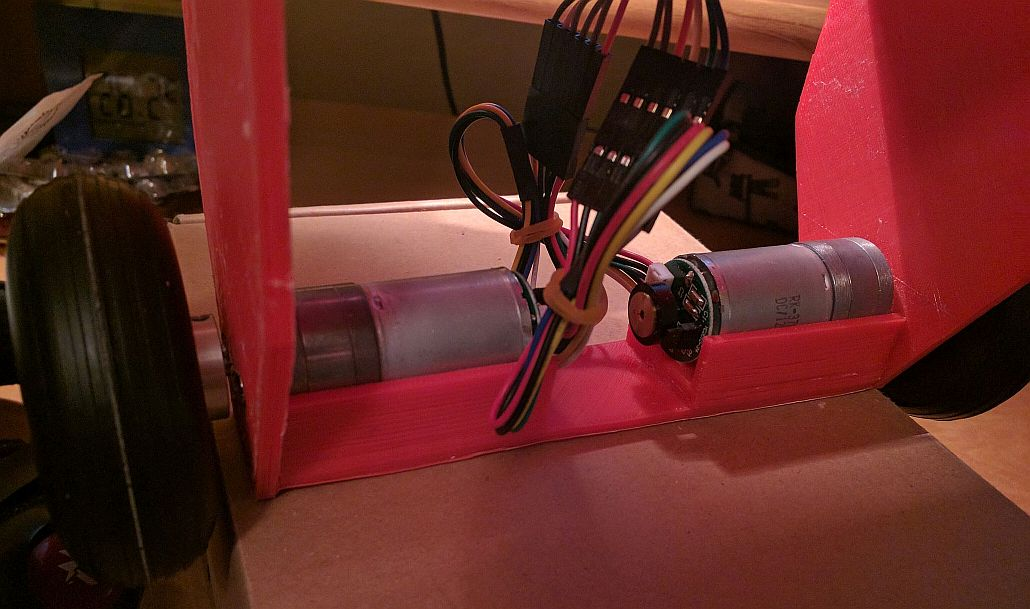
\includegraphics[scale=0.4]{\ImgPath/silnikidc.jpg}
\end{center}
	\caption{Silnik DC Pololu 12 V [opracowanie własne]}
	\label{schematKomunikacji}
\end{figure}

\newpage
\noindent Do wału silnika zostały dopasowane łożyska kulkowe o średnicach 4 mm i 12 mm oraz grubości 4 mm. Dzięki nim następuje bezpieczniejsze przełożenie napędu na koła z minimalnym tarciem. Obniżają nacisk na wał silnika.

\begin{figure}[!htbp]
	\begin{center}
\centering
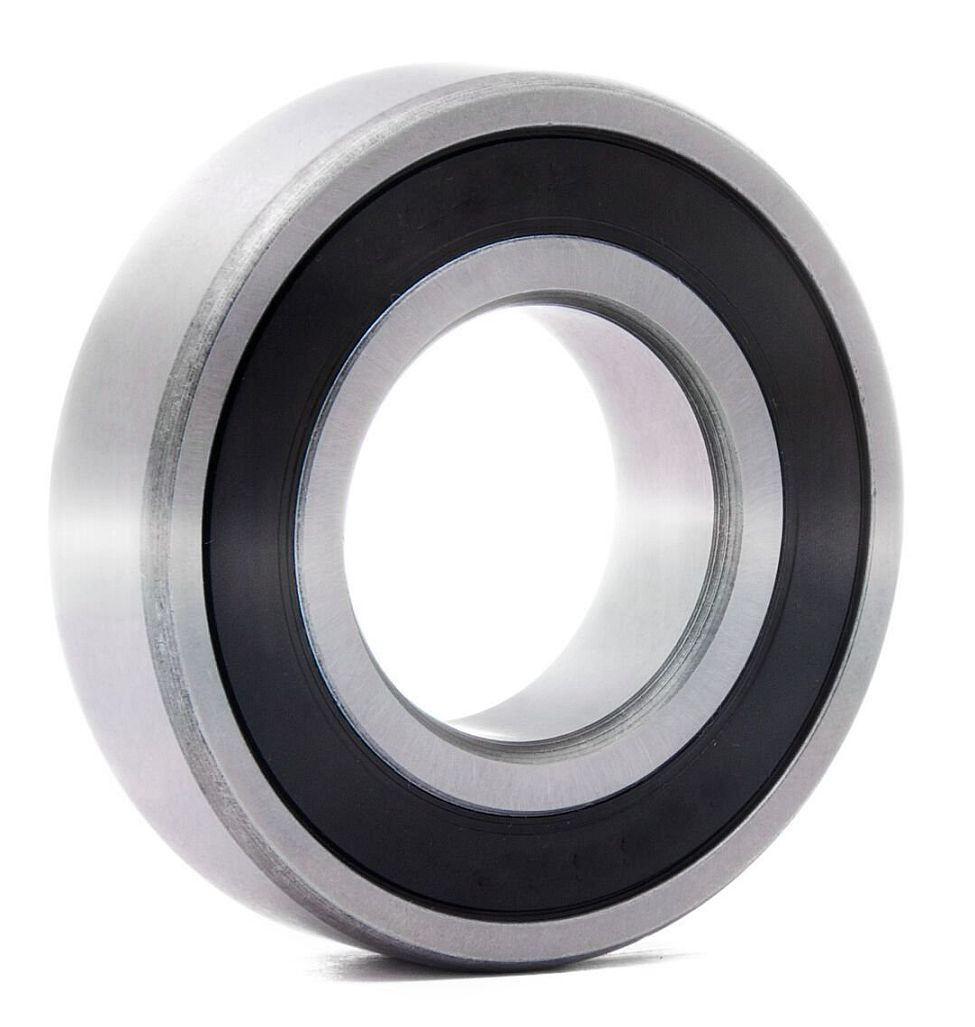
\includegraphics[scale=0.1]{\ImgPath/lozysko.jpg}
\end{center}
	\caption{Łożysko kulkowe [źródło: www.allegro.pl, aukcja sklepu TECH-POL-net]}
	\label{schematKomunikacji}
\end{figure}
 
  %-----------------
  % Koła
  %-----------------
\section{Koła}

W konstrukcji zostały użyte lekkie poliuretanowe koła z plastikową piastą, charakteryzują się niską ceną i dostateczną przyczepnością.\\
Parametry koła:
\begin{itemize}
\item średnica opony: 70 mm,
\item szerokość opony: 24 mm ,
\item średnica otworu: 4 mm ,
\item średnica plastikowej piasty: 35 mm ,
\item waga: 30g.
\end{itemize}

Do połączenia kół z krótkim wałem silnika zostały skonstruowane specjalne łączniki na śruby. Ich działanie polega na zaciśnięciu bocznej śruby o średnicy 2,5 mm do granic możliwości. Wymagane jest w tym momencie specjalne ułożenie, w środku łącznika, wału silnika, którego przekrój nie jest idealnym okręgiem, lecz zawiera delikatne zeszlifowanie (kształtem przypomina literę D). Po dociśnięciu śruby w miejsce tego szlifu jakikolwiek luz zostanie wyeliminowany.

\begin{figure}[!htbp]
	\begin{center}
\centering
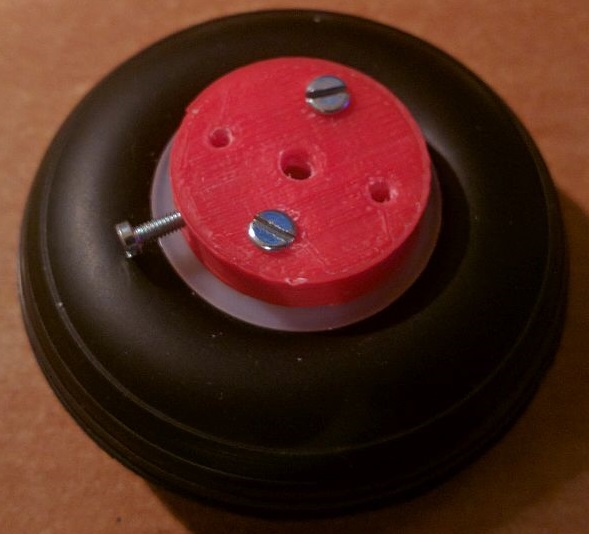
\includegraphics[scale=0.3]{\ImgPath/hub.jpg}
\end{center}
	\caption{Hub mocujący wał silnika z kołem [opracowanie własne]}
	\label{schematKomunikacji}
\end{figure}

Po testach wytrzymałościowych okazało się, że plastikowe tworzywo ABS nie wytrzymało dużych naprężeń śruby na wał silnika i uległo odkształceniu, dlatego zostały zastosowane uniwersalne aluminiowe huby mocujące z otworem na 4 mm.

\begin{figure}[!htbp]
	\begin{center}
\centering
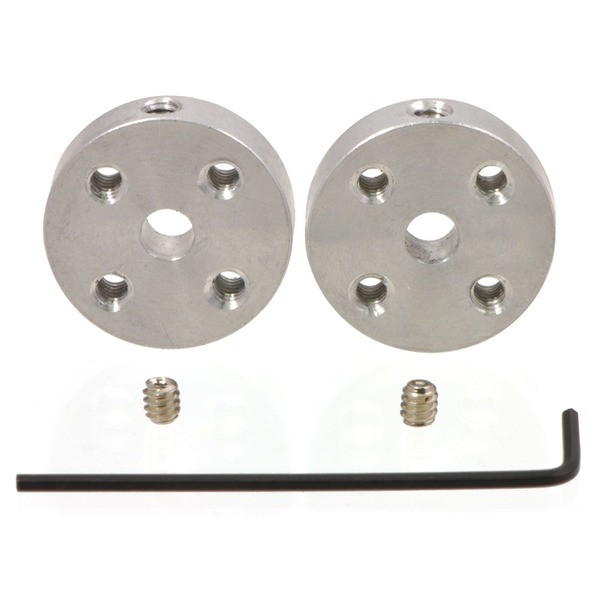
\includegraphics[scale=0.35]{\ImgPath/huby.jpg}
\end{center}
	\caption{Aluminiowy hub mocujący [źródło: https://botland.com.pl/6039-thickbox\_default/aluminiowy-hub-mocujacy-4mm-m3-2-szt.jpg]}
	\label{schematKomunikacji}
\end{figure}

  %-----------------
  % Matematyczny model układu
  %-----------------
\section{Matematyczny model układu}

Robot jest zbudowany symetrycznie w odniesieniu do szerokości i długości, więc po zastosowaniu uproszczenia środek masy jedynie w odniesieniu do wysokości wymaga przeprowadzenia dokładnych obliczeń. Reszta wartości będzie się pokrywała ze środkiem geometrycznym bryły. Przy obliczeniach położenie i masa przewodów zostały ujęte w dużym przybliżeniu.\\

Środek masy i moment bezwładności zostały obliczone poprzez podzielenie robota na obiekty i wyliczenie dla każdego środka masy i momentu bezwładności, a następnie zsumowanie wszystkich składowych w programie Microsoft Excel 2013.

\begin{figure}[!htbp]
	\begin{center}
\centering
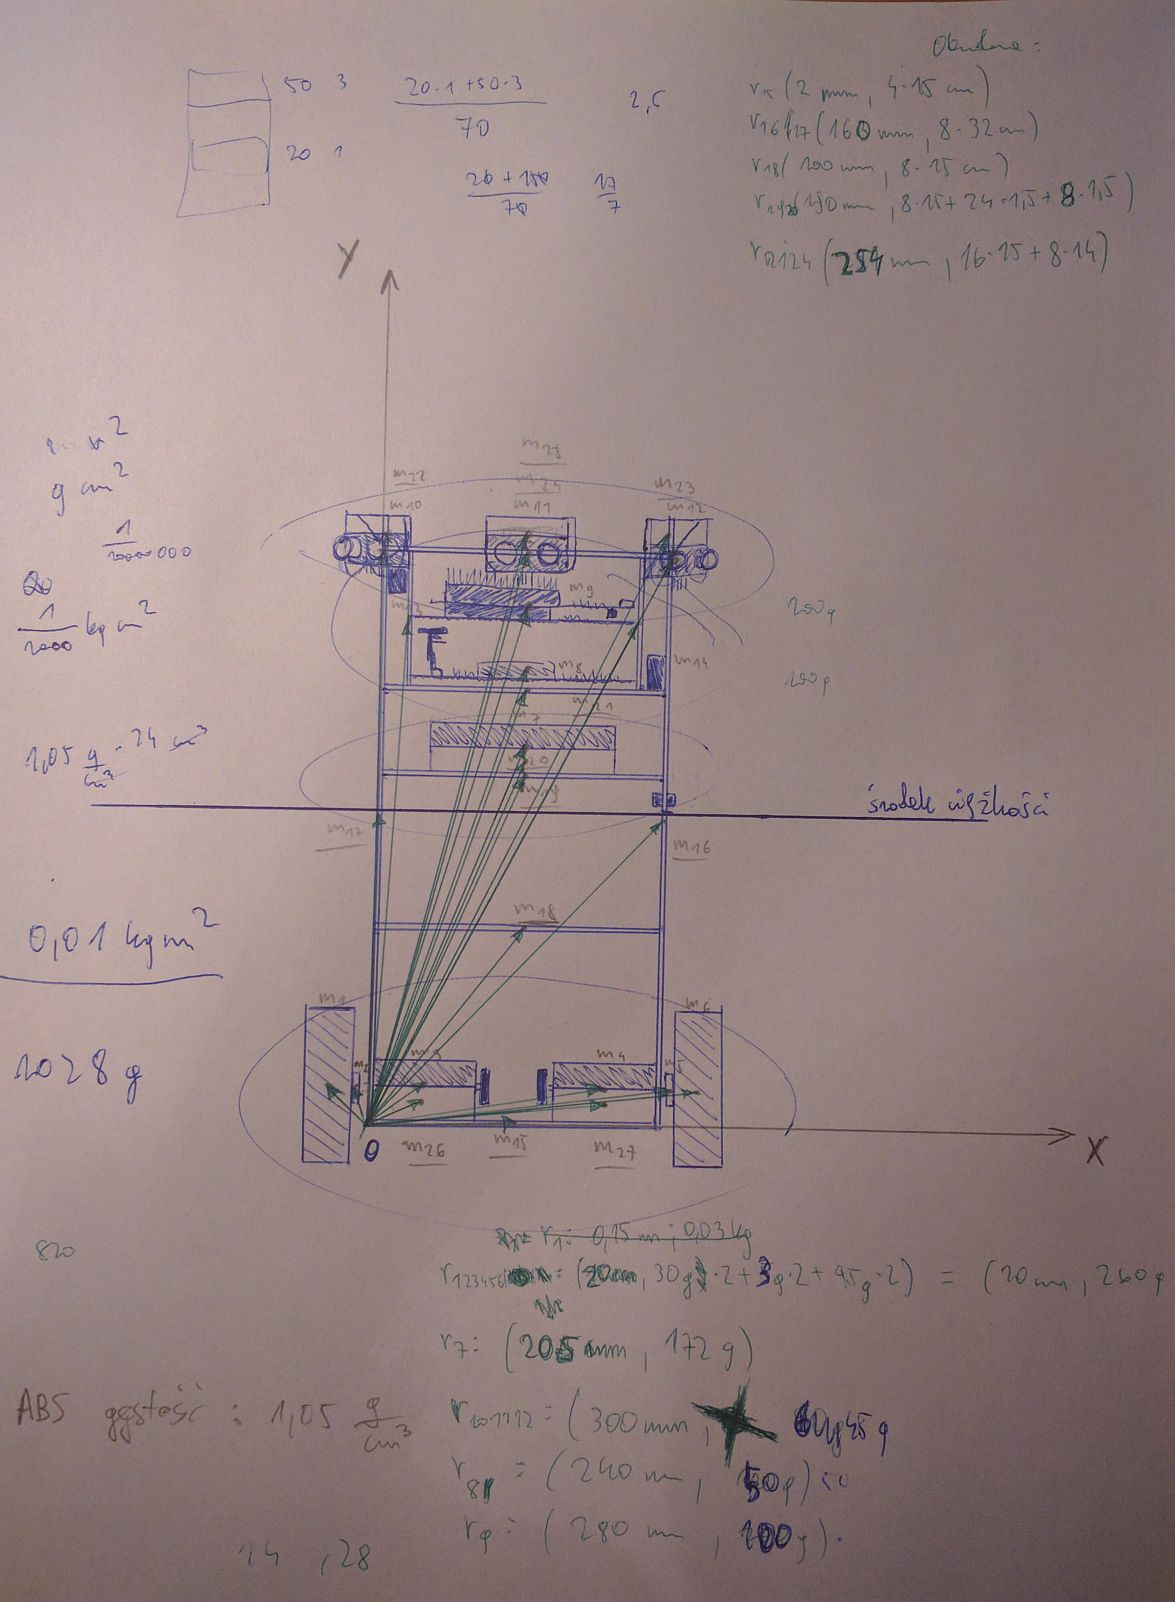
\includegraphics[scale=0.3]{\ImgPath/wektory.jpg}
\end{center}
	\caption{Wektory środków geometrycznych poszczególnych obiektów [opracowanie własne]}
	\label{schematKomunikacji}
\end{figure}
\newpage
\noindent Obliczone dane bryły:
\begin{itemize}
\item wysokość środka masy obudowy: 162.6 mm,
\item moment bezwładności obudowy: 0.01 $kg*m^2$.
\end{itemize}

\noindent Obliczenia wykonane w programie Microsoft Excel 2013:

\begin{figure}[!htbp]
	\begin{center}
\centering
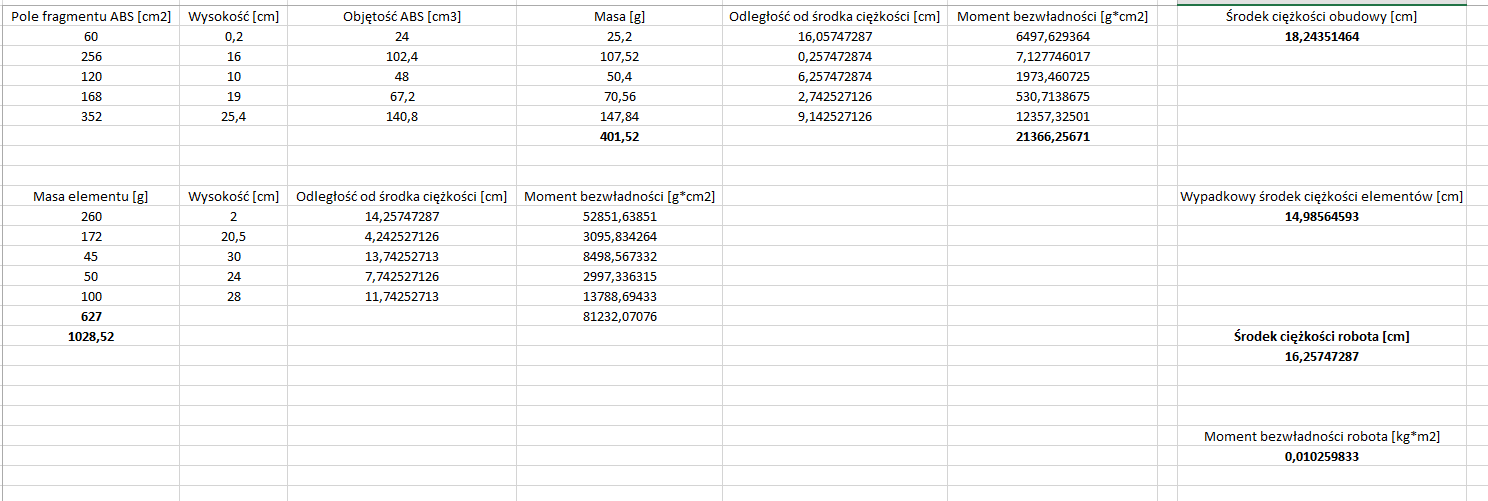
\includegraphics[scale=0.32]{\ImgPath/i.PNG}
\end{center}
	\caption{Obliczenie środka ciężkości i momentu bezwładności robota w programie Microsoft Excel 2013 [opracowanie własne]}
	\label{schematKomunikacji}
\end{figure}

\newpage
  %-----------------
  % Wyznaczenie równań liniowych układu
  %-----------------
\section{Wyznaczenie równań liniowych układu}


Jest to układ odwróconego wahadła, który przypomina patyk znajdujący się na wózku, na który działa siła z zewnątrz. Układ taki wygląda następująco:\\

\begin{figure}[!htbp]
	\begin{center}
\centering
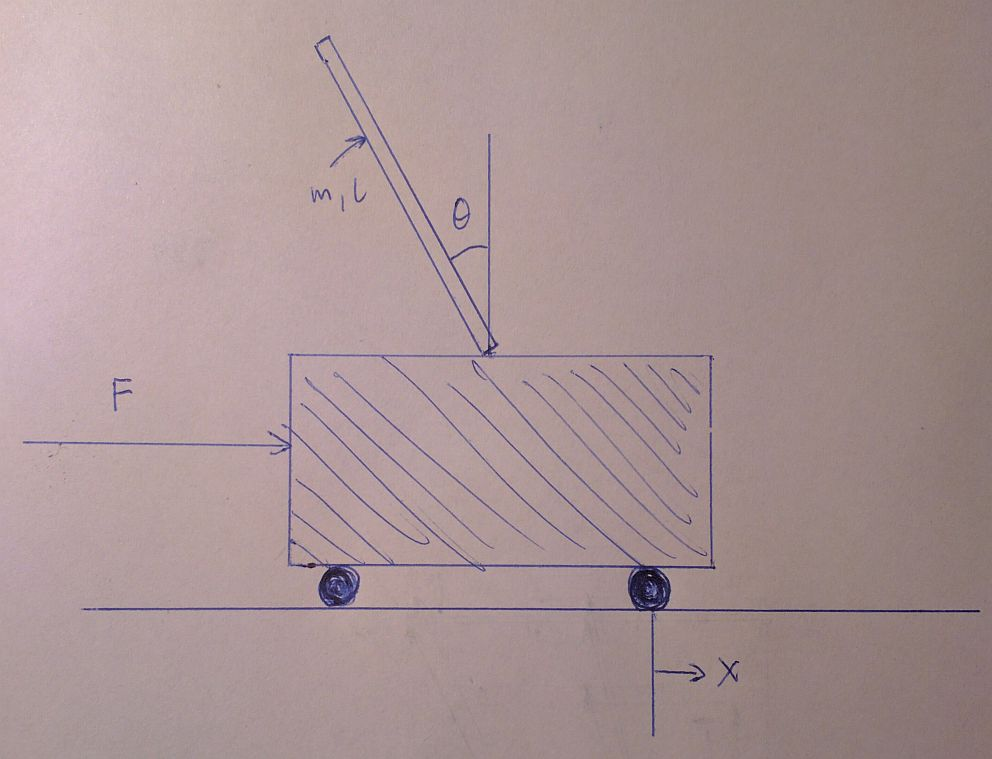
\includegraphics[scale=0.2]{\ImgPath/wahadlo.jpg}
\end{center}
	\caption{Układ wahadła odwróconego [opracowanie własne]}
	\label{schematKomunikacji}
\end{figure}

\noindent Równania opisujące model:\\
\\
$F=(M+m)\ddot{x}+b\dot{x}+ml\ddot{\theta}cos\theta-ml\dot{\theta}^2sin\theta$ \\
$-ml\ddot{x}cos\theta=(I+ml^2)\ddot{\theta}+mglsin\theta$ \\
\\
Dane układu:
\begin{itemize}
\item M - masa wózka: 0 kg (wózek słuzył tylko do zilustrowania sytuacji),
\item m - masa odwróconego wahadła: 1 kg,
\item I - moment bezwładności odwróconego wahadła: 0.01 $kgm^2$,
\item F - siła działająca na wózek: nie większa niż 4 N (założenie),
\item x - położenie wózka - zmienna stanu mierzona w metrach,
\item $\theta$ - wychylenie wahadła od pionu - zmienna stanu mierzona w stopniach,
\item b - współczynnik tarcia wózka o podłoże: ok. 0.1 N/m/s, 
\item l - odległość od środka masy: 0.137 m,
\item g - przyspieszenie ziemskie w Warszawie: 9.8123 m/$s^2$.
\end{itemize} 

\noindent W przypadku robota balansującego na dwóch kołach równanie upraszacza się do postaci:\\
\\
$F=m\ddot{x}+b\dot{x}+ml\ddot{\theta}cos\theta-ml\dot{\theta}^2sin\theta$ \\
$-ml\ddot{x}cos\theta=(I+ml^2)\ddot{\theta}+mglsin\theta$ \\
\\
Powyższe równania są nieliniowe, więc po linearyzacji w otoczeniu punktu $\theta=\pi$ otrzymaNO następujące równania ($\theta=\pi+\phi$, gdzie $\phi$ reprezentuje małe odchylenia wahadła, a u to wejście układu):\\
\\
$u=m\ddot{x}+b\dot{x}-ml\ddot{\phi}$ \\
$ml\ddot{x}=(I+ml^2)\ddot{\phi}-mgl\phi$ \\

\noindent Opis układu w przestrzeni zmiennych stanu:\\
\\
\noindent $\dot{x}=Ax+Bu$ \\
$y=Cx+Du$ \\
\\
\\$
     \begin{bmatrix}
       \dot{x} \\
       \ddot{x} \\
       \dot{\phi} \\
       \ddot{\phi}
     \end{bmatrix}
     =
     \begin{bmatrix}
       0 & 1 & 0 & 0          \\
       0 & \frac{-(I+ml^2)b}{Im} & \frac{mgl^2}{I} & 0 \\
       0 & 0 & 0 & 1 \\
       0 & \frac{-lb}{I} & \frac{mgl}{I} & 0 
     \end{bmatrix}
     \begin{bmatrix}
       x \\
       \dot{x} \\
       \phi \\
       \dot{\phi}
     \end{bmatrix}
     +
     \begin{bmatrix}
       0 \\
       \frac{I+ml^2}{Im} \\
       0 \\
       \frac{l}{I}
     \end{bmatrix}
     u\\
     y=
     \begin{bmatrix}
       1 & 0 & 0 & 0 \\
       0 & 0 & 1 & 0 
     \end{bmatrix}
     \begin{bmatrix}
       x \\
       \dot{x} \\
       \phi \\
       \dot{\phi}
     \end{bmatrix}
     +
     \begin{bmatrix}
       0 \\
       0 
     \end{bmatrix}
     u
$
\\
\\

\noindent Po wstawieniu liczb:\\
\\$
     \begin{bmatrix}
       \dot{x} \\
       \ddot{x} \\
       \dot{\phi} \\
       \ddot{\phi}
     \end{bmatrix}
     =
     \begin{bmatrix}
       0 & 1 & 0 & 0          \\
       0 & -0.2877 & 18.4167 & 0 \\
       0 & 0 & 0 & 1 \\
       0 & -1.37 & 134.4285 & 0 
     \end{bmatrix}
     \begin{bmatrix}
       x \\
       \dot{x} \\
       \phi \\
       \dot{\phi}
     \end{bmatrix}
     +
     \begin{bmatrix}
       0 \\
       2.8769 \\
       0 \\
       13.7
     \end{bmatrix}
     u\\
     y=
     \begin{bmatrix}
       1 & 0 & 0 & 0 \\
       0 & 0 & 1 & 0 
     \end{bmatrix}
     \begin{bmatrix}
       x \\
       \dot{x} \\
       \phi \\
       \dot{\phi}
     \end{bmatrix}
     +
     \begin{bmatrix}
       0 \\
       0 
     \end{bmatrix}
     u
$


\chapter{Elektronika}

  %-----------------
  % Zasilanie
  %-----------------
\section{Zasilanie}

\subsection{Akumulator}

Do zasilania został użyty pakiet ogniw litowo-polimerowych firmy Redox. Akumulator został wybrany ze względu na to, że dostarcza dużo energii przy małych rozmiarach, a także może być stale obciążony dużym prądem. \\
Dane techniczne:
\begin{itemize}
\item napięcie nominalne: 11,1 V (pełne naładowanie - 12,6 V),
\item pojemność: 2200 mAh,
\item prąd rozładowania: 30 C (66 A),
\item wymiary: 115 x 34 x 20 mm,
\item masa: 172 g.
\end{itemize}

W najbardziej pesymistycznym przypadku robot może pobierać do 5 A ciągłego prądu. Przy pojemności 2200 mAh daje to minimalny czas pracy około 26 minut. Natomiast w przypadku zwykłej jazdy, bez przeszkód robot może pobrać ok. 1 A, co przekłada się na pięciokrotnie dłuższe działanie. W 130 minut powinno dać się zmapować kilka razy w ciągu nocy całe piętro budynku.

\begin{figure}[!htbp]
	\begin{center}
\centering
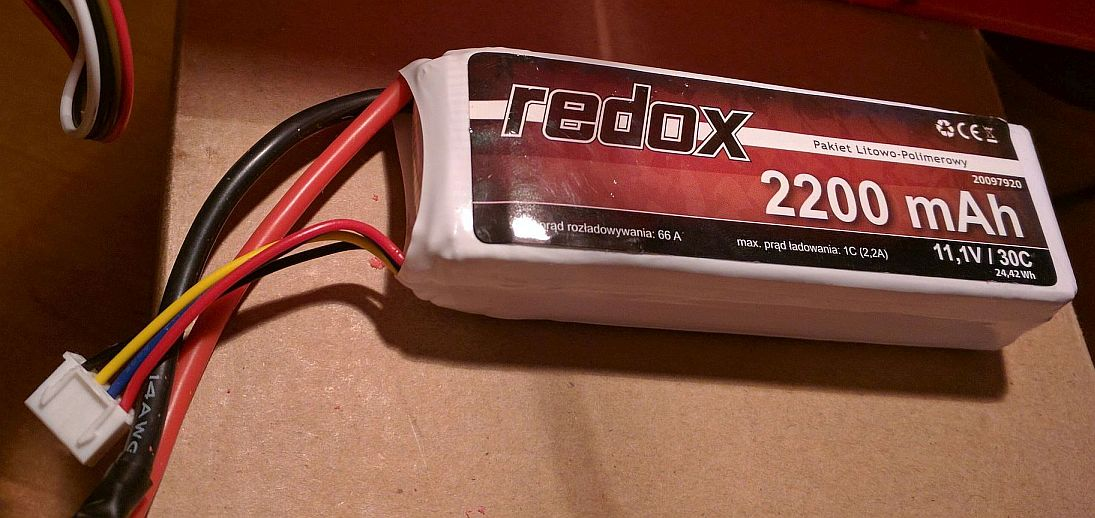
\includegraphics[scale=0.4]{\ImgPath/lipo.jpg}
\end{center}
	\caption{Akumulator litowo-polimerowy firmy Redox [opracowanie własne]}
	\label{schematKomunikacji}
\end{figure}

\newpage

Napięcie z akumulatora jest bezpośrednio przekazywane tylko do silników (na dwukanałowy mostek), a na układy logiczne dostarczane jest poprzez stabilizatory liniowe 7805 na 5 V i LD1117VC33 na 3.3 V. Stabilizatory są w obudowach TO-220, co ułatwia ich chłodzenie. Zasilają części logiczne, więc wbudowana blaszka odprowadzająca ciepło wystarczy, żeby cały układ się nie przegrzał. Do stabilizatorów zostały dołączone kondensatory MKT 330 nF i ceramiczne 100 nF zgodnie z notą katalogową.

\begin{figure}[!htbp]
	\begin{center}
\centering
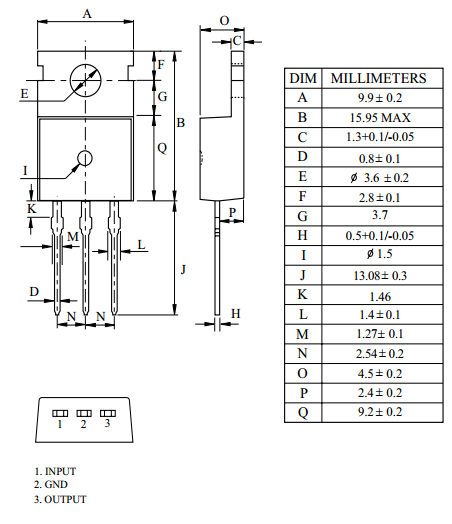
\includegraphics[scale=0.4]{\ImgPath/7805.PNG}
\end{center}
	\caption{Układ 7805 [źródło: bibliografia pkt. 1, strona 1]}
	\label{schematKomunikacji}
\end{figure}
\newpage
\begin{figure}[!htbp]
	\begin{center}
\centering
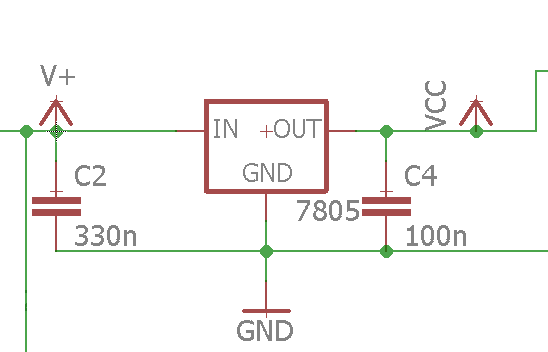
\includegraphics[scale=0.4]{\ImgPath/7805e.PNG}
\end{center}
	\caption{Schemat połączeń układu 7805, program EAGLE [opracowanie własne]}
	\label{schematKomunikacji}
\end{figure}

\begin{figure}[!htbp]
	\begin{center}
\centering
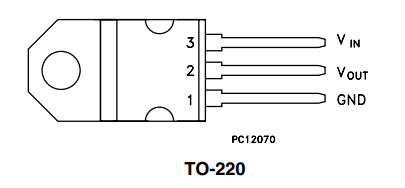
\includegraphics[scale=0.6]{\ImgPath/ld1117.PNG}
\end{center}
	\caption{Układ LD1117VC33 [źródło: bibliografia pkt. 2, strona 3]}
	\label{schematKomunikacji}
\end{figure}

\begin{figure}[!htbp]
	\begin{center}
\centering
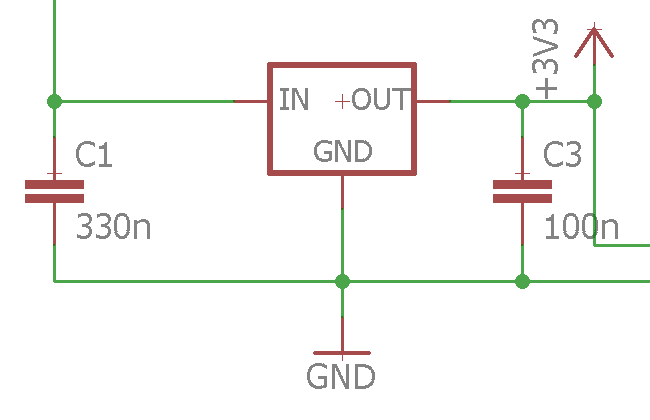
\includegraphics[scale=0.4]{\ImgPath/ld1117e.PNG}
\end{center}
	\caption{Schemat połączeń układu LD1117VC33, program EAGLE [opracowanie własne]}
	\label{schematKomunikacji}
\end{figure}

\newpage

Napięcie 5 V jest kierowane do sterownika silników z mikrokontrolerem ATmega168PA-PU, a także do zasilania płytki NUCLEO z mikrokontrolerem STM32F103RBT6. Napięcie 3,3 V służy do zasilenia niektórych czujników i układów, na przykład modułu WiFi ESP8266.

\subsection{Ładowarka}

Ładowanie pakietów ogniw litowo-polimerowych wymaga stosowania ładowarek mikroprocesorowych z odpowiednim algorytmem ładowania, wyposażonych w układy balancerów, które równomiernie ładują każde ogniwo. W celu uniknięcia trwałych uszkodzeń ogniwa powinno się nie rozładowywać go poniżej 3V, czyli w przypadku całego pakietu napięcie nie powinno osiągnąć wartości poniżej 9 V.

W celu zachowania powyższych zasad została zastosowana ładowarka sieciowa firmy Redox. Specyfikacja:
\begin{itemize}
\item Napięcie wejściowe: 100 - 240 V AC 50 / 60 Hz,
\item Prąd ładowania: do 1000 mA,
\item Obsługiwane pakiety: 2-3 ogniwowe litowo-polimerowe (7,4  V i 11,1 V),
\item Wbudowany balancer ogniw,
\item Długość przewodów: 150 cm,
\item Wymiary: 96 x 55 x 33 mm.
\end{itemize}

\begin{figure}[!htbp]
	\begin{center}
\centering
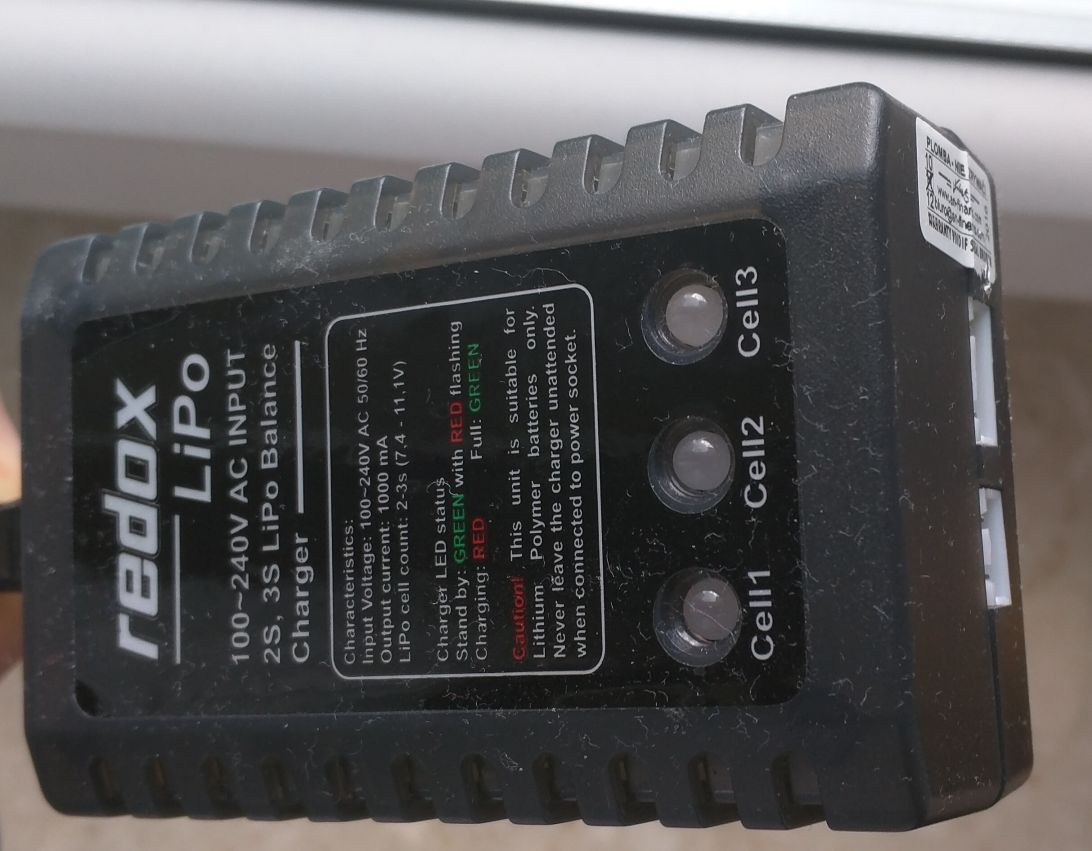
\includegraphics[scale=0.22]{\ImgPath/ladowarka.jpg}
\end{center}
	\caption{Ładowarka sieciowa Redox [opracowanie własne]}
	\label{schematKomunikacji}
\end{figure}

\section{Zabezpieczenie elektroniki}

Elektronika może ulec uszkodzeniu ze względu na wiele czynników: silne pole magnetyczne, wysoka temperatura, za duży prąd lub napięcie. W układzie zostało zastosowanych kilka zabezpieczeń:
\begin{itemize}
\item Akumulator jest podłączony do przełącznika na prąd do 15 A, który służy jako główny włącznik robota,
\item Dodatni sygnał z akumulatora przechodzi przez szeregowo wpięty rezystor 0,1~$\Omega$ 5 W, który ogranicza przepływ prądu do 7 A, ze względu na swoją wytrzymałość. Służy on również do pomiaru prądu przez przetwornik analogowo-cyfrowy mikrokontrolera ATMega168PA-PU, jeżeli prąd osiągnie kosztownie wysoką wartość, to układ scalony ma możliwość obniżenia go do bezpiecznej normy,
\item do dwukanałowego mostka w sterowniku silników, został dołączony radiator w formie dwóch lekkich blaszek aluminiowych (fragmentów ościeżnicy)
\end{itemize}

  %-----------------
  % Sterownik silników prądu stałego
  %-----------------
\section{Sterownik silników prądu stałego}

Do sterowania silników DC został wybrany mikrokontroler ATmega168PA-PU w obudowie DIP28. Sterowanie odbywa się za pomocą nadawania sygnału PWM na piny dwukanałowego mostka L298N. Do układu mostków i mikrokontrolera zostały dołączone filtry poprzez umieszczenie kondensatorów i dławików zgodnie z notami katalogowymi. Dodatkowo do L298N zostały dołączone diody, które były wymagane do prawidłowego działania układu. \\
Do łatwego przeprogramowywania mikrokontrolera na płytce znajduje się złącze programatora zgodnego z USBASP o 10 pinowym standardzie KANDA.

\begin{figure}[!htbp]
	\begin{center}
\centering
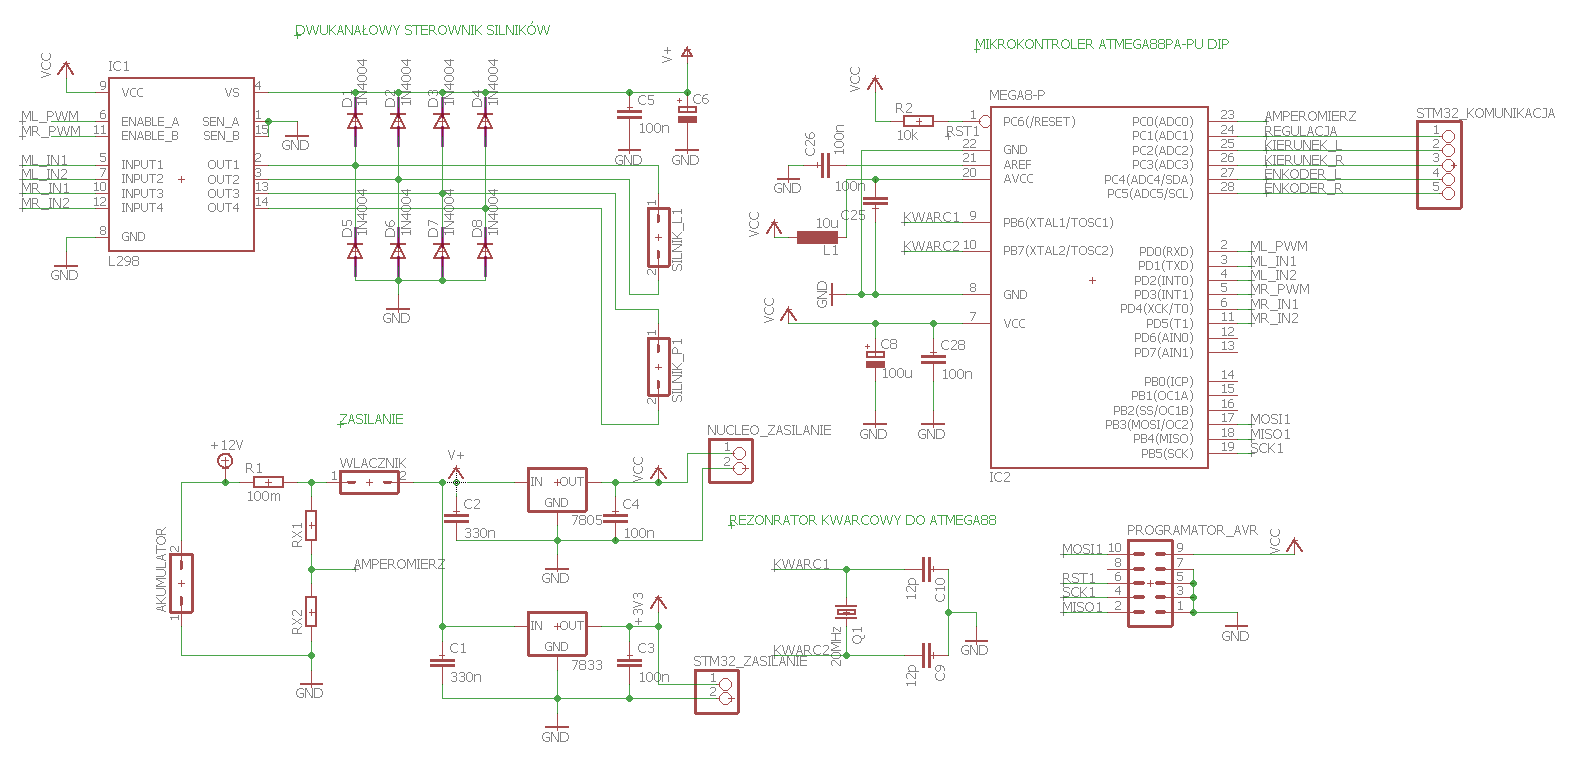
\includegraphics[scale=0.33]{\ImgPath/silnikie.PNG}
\end{center}
	\caption{Sposób połączenia elementów elektronicznych sterownika silników prądu stałego wykonany w programie Cadsoft EAGLE [opracowanie własne]}
	\label{schematKomunikacji}
\end{figure}

\newpage

\subsection{Mikrokontroler ATMega168PA-PU}

Mikrokontroler ATMega168PA-PU 8-bitowy z rodziny AVR w obudowie DIP28 został wybrany ze względu na niskie zapotrzebowanie mocy obliczeniowej w układzie sterownika silników, a co się z tym wiąże układ może być bardzo tani.\\
Dane techniczne:
\begin{itemize}
\item taktowanie: do 20 MHz,
\item pamięć Flash: 16 kB,
\item pamięć RAM: 1 kB,
\item 23 linie wyjścia/wejścia,
\item 2 timery 8-bitowe,
\item 1 timer 16-bitowy,
\item 6 kanałów 10-bitowego przetwornika analogowo-cyfrowego,
\item sprzętowe interfejsy komunikacyjne: USART, SPI, 2-wire (I2C).
\end{itemize}

\begin{figure}[!htbp]
	\begin{center}
\centering
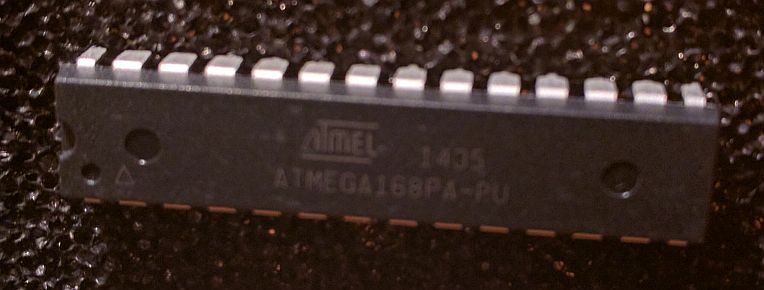
\includegraphics[scale=0.2]{\ImgPath/atmega.jpg}
\end{center}
	\caption{Mikrokontroler ATMega168PA-PU w obudowie DIP28 [opracowanie własne]}
	\label{schematKomunikacji}
\end{figure}

\begin{figure}[!htbp]
	\begin{center}
\centering
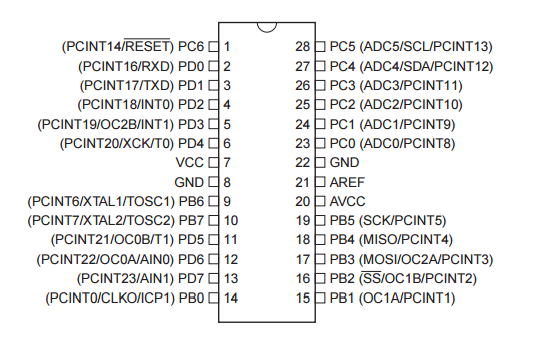
\includegraphics[scale=0.7]{\ImgPath/atmegapins.PNG}
\end{center}
	\caption{Rozkład pinów ATMega168PA-PU w obudowie DIP28 [źródło: bibliografia pkt. 3, strona 2]}
	\label{schematKomunikacji}
\end{figure}

\begin{figure}[!htbp]
	\begin{center}
\centering
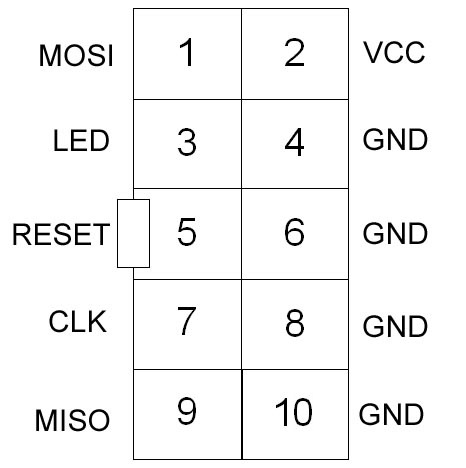
\includegraphics[scale=0.3]{\ImgPath/kanda.jpg}
\end{center}
	\caption{Schemat gniazda KANDA (złącze programatora mikrokontrolera ATMega168PA-PU) [opracowanie własne]}
	\label{schematKomunikacji}
\end{figure}

\begin{figure}[!htbp]
	\begin{center}
\centering
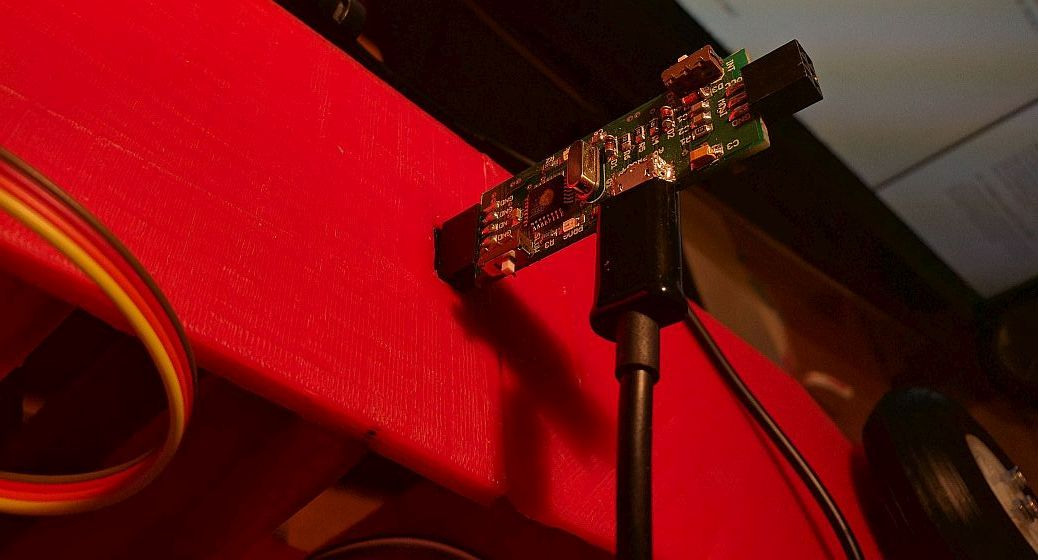
\includegraphics[scale=0.4]{\ImgPath/programatoravr.jpg}
\end{center}
	\caption{Gniazdo programatora AVR wbudowane w obudowę robota [opracowanie własne]}
	\label{schematKomunikacji}
\end{figure}

\newpage

Mikrokontroler jest programowany poprzez dzisięciopinowe gniazdo KANDA połączone z programatorem zgodnym z USBasp. Programator ma wyjście Mini USB, co pozwala na bezproblemowe podłączenie do komputera PC.\\
Do prawidłowego działania układu wymaganych jest kilka dodatkowych elementów, zgodnie z notą katalogową:
\begin{itemize}
\item kondensatory ceramiczne 100 nF między piny AREF a GND, VCC a GND i AVCC a GND,
\item kondensator elektrolityczny \SI{100}{\micro F} 16 V między piny VCC a GND,
\item dławik \SI{10}{\micro H} między piny AVCC i VCC,
\item rezystor 10 $k\Omega$ 0,25 W podciągający pin RESET do VCC,
\item rezonator kwarcowy 20 MHz do pinów XTAL1 i XTAL2 z dołączonymi kondensatorami ceramicznymi 12 pF.
\end{itemize}

\newpage

\begin{figure}[!htbp]
	\begin{center}
\centering
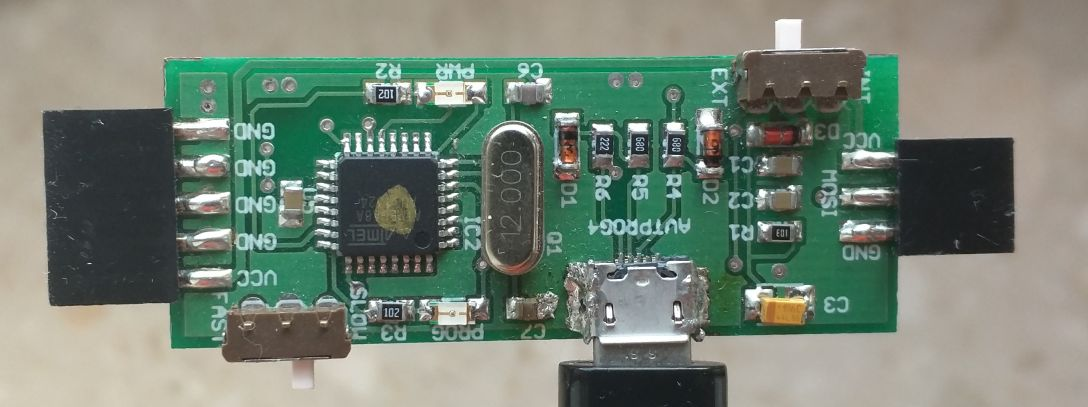
\includegraphics[scale=0.3]{\ImgPath/usbasp.jpg}
\end{center}
	\caption{Wykorzystany programator zgodny z USBasp [opracowanie własne]}
	\label{schematKomunikacji}
\end{figure}

Układ ATMega168PA-PU jest wykorzystywany do sterowania prędkościami silników za pomocą regulatora PID i sprzężenia zwrotnego w postaci odczytu położenia kół z enkoderów magnetycznych znajdujących się przy silnikach. Wartość zadana skorygowana o uchyb jest przekazywana w postaci sygnału PWM na wejścia dwukanałowego mostka H w postaci układu scalonego L298N. Na przetwornik analogowo cyfrowy ADC0 jest podawane napięcie na rezystorze wejściowym 0,1 $\Omega$ wpiętym szeregowo przy dodatnim złączu akumulatora, co pozwala na pomiar całkowitego prądu płynącego w układzie. W przypadku osiągnięcia dużych wartości, pobór prądu zostanie programowo zmniejszony. Mikrokontroler zawiera również kilka połączeń z drugim mikrokontrolerem STM32F103RBT6 za pomocą pinów PC1-PC3, zawierających informacje o kierunku i szybkości jazdy.

\newpage

\begin{figure}[!htbp]
	\begin{center}
\centering
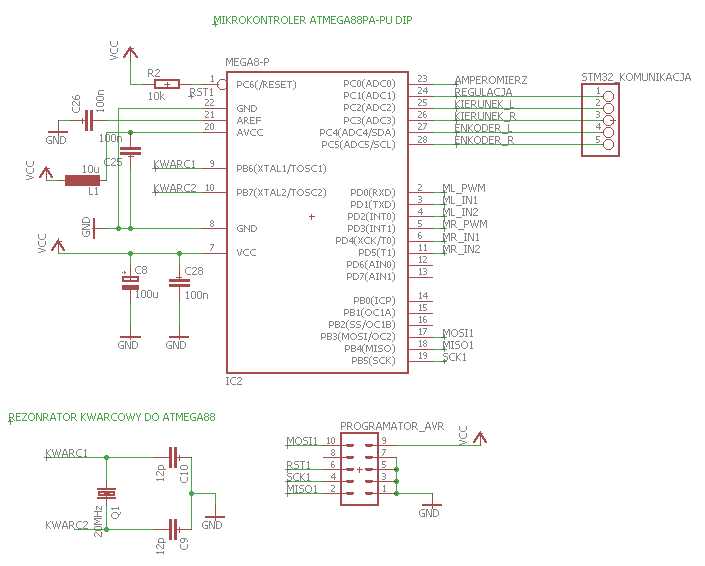
\includegraphics[scale=0.7]{\ImgPath/atmegapol.PNG}
\end{center}
	\caption{Sposób połączenia mikrokontrolera ATMega168PA-PU wykonany w programie EAGLE [opracowanie własne]}
	\label{schematKomunikacji}
\end{figure}

\subsection{Dwukanałowy mostek H - układ L298N}

Sam układ scalony L298N, nie w gotowym module, został zastosowany ze względu na niewielką cenę. Do prawidłowego działania należało jedynie dokupić, według noty katalogowej, 8 diod prostowniczych, 1 kondensator elektrolityczny \SI{100}{\micro F} i 1 kondensator ceramiczny 100 nF.

\begin{figure}[!htbp]
	\begin{center}
\centering
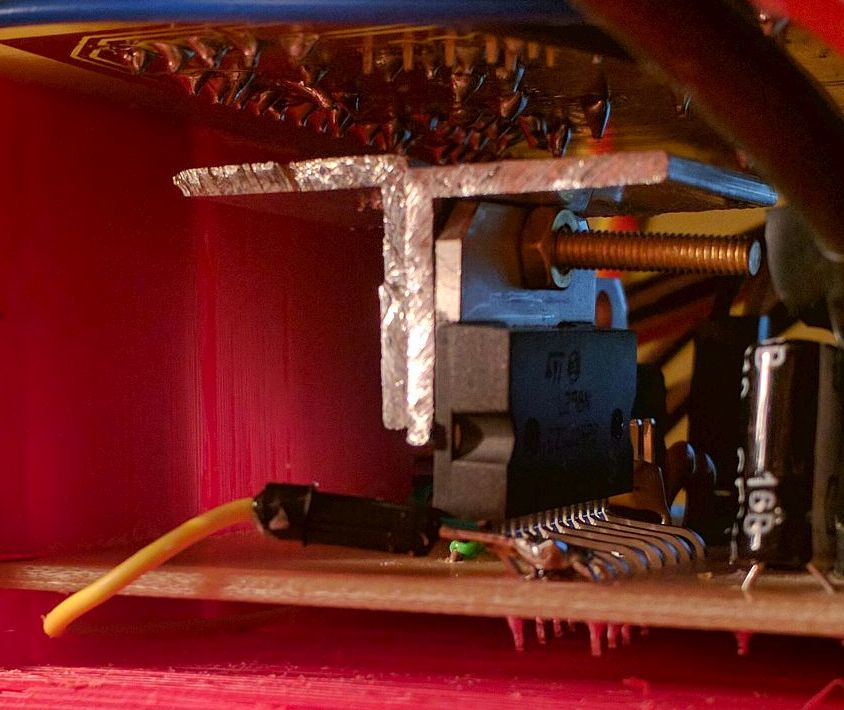
\includegraphics[scale=0.3]{\ImgPath/l298n.jpg}
\end{center}
	\caption{Układ scalony L298N z aluminiowymi radiatorami [opracowanie własne]}
	\label{schematKomunikacji}
\end{figure}

\begin{figure}[!htbp]
	\begin{center}
\centering
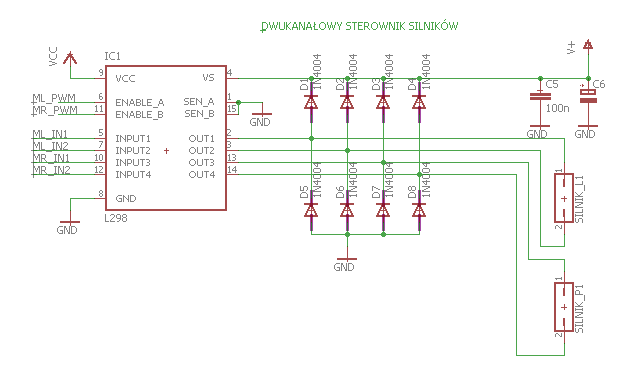
\includegraphics[scale=0.7]{\ImgPath/l298npol.PNG}
\end{center}
	\caption{Schemat połączenia układu L298N wykonany w programie EAGLE [opracowanie własne]}
	\label{schematKomunikacji}
\end{figure}

\newpage

\subsection{Enkodery magnetyczne CPR 48}

Zastosowane enkodery są zintegrowane z używanymi silnikami. Ich działanie jest oparte na zjawisku Halla - sensory wykrywają impulsy na obracającej się tarczy magnetycznej umieszczonej z tyłu silnika. Używane enkodery kwadraturowe posiadają rozdzielczość 48 impulsów na obrót, co po przemnożeniu przez wartość przekładni 9,7:1 - daje wynik prawie 466 impulsów na obrót.

\begin{figure}[!htbp]
	\begin{center}
\centering
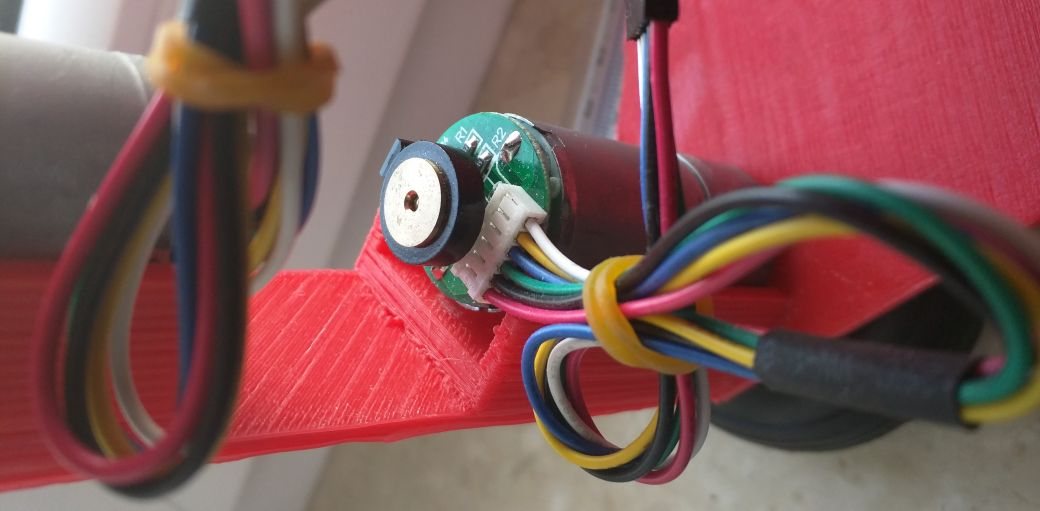
\includegraphics[scale=0.4]{\ImgPath/enkoder.jpg}
\end{center}
	\caption{Enkodery magnetyczne CPR 48 i wyprowadzenia przewodów silnika [opracowanie własne]}
	\label{schematKomunikacji}
\end{figure}

Wyprowadzenia silników:
\begin{itemize}
\item czerwony - zasilanie silnika 1,
\item czarny - zasilanie silnika 2,
\item zielony - potencjał masy enkodera,
\item niebieski - zasilanie enkodera, tolerancja od 3.5 V do 20 V,
\item żółty - wyjście A enkodera,
\item biały - wyjście B enkodera,
\end{itemize}

\newpage

\subsection{Wykonanie płytki PCB}

Oprócz schematu połączeń elementów elektronicznych w programie EAGLE został również wykonany projekt płytki PCB:

\begin{figure}[!htbp]
	\begin{center}
\centering
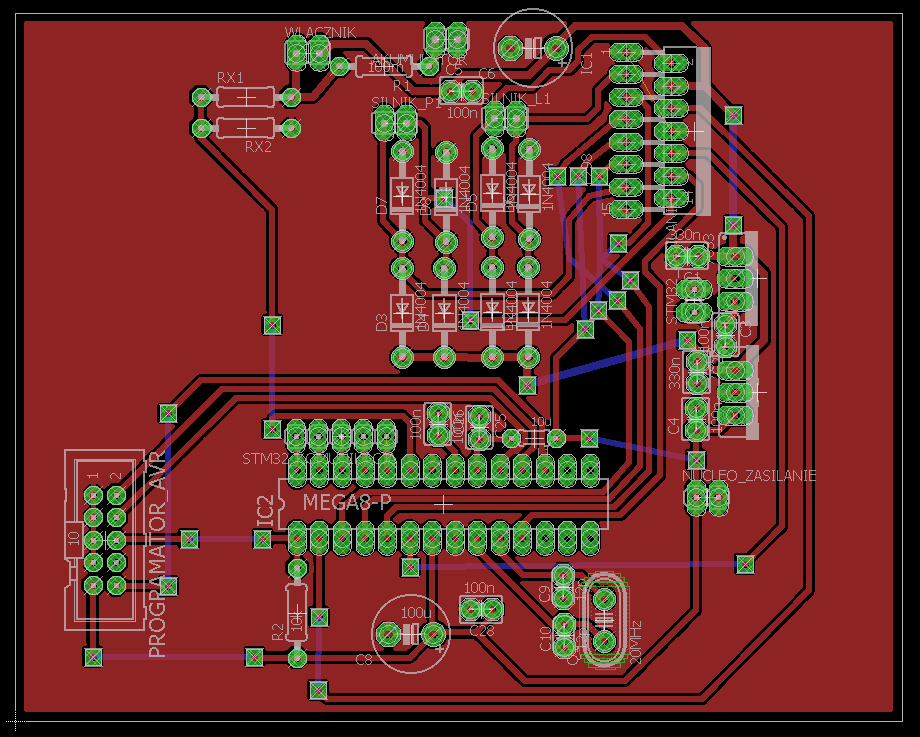
\includegraphics[scale=0.35]{\ImgPath/silnikip.PNG}
\end{center}
	\caption{Projekt płytki PCB sterownika silników prądu stałego wykonany w programie Cadsoft EAGLE [opracowanie własne]}
	\label{schematKomunikacji}
\end{figure}

\begin{figure}[!htbp]
	\begin{center}
\centering
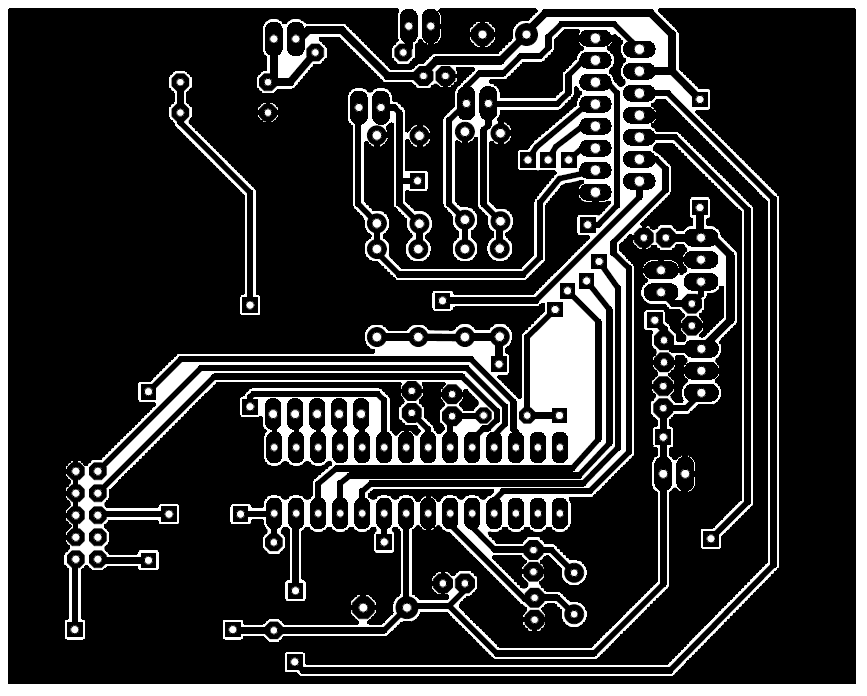
\includegraphics[scale=0.35]{\ImgPath/silnikid.PNG}
\end{center}
	\caption{Obraz połączeń elementów elektronicznych sterownika silników prądu stałego przygotowany do wydrukowania [opracowanie własne]}
	\label{schematKomunikacji}
\end{figure}

\newpage
Projekt płytki PCB został wyeksportowany do pliku PDF, aby uniknąć jakiegokolwiek przeskalowania elementów. Wydruk został przeprowadzony na drukarce laserowej na papierze kredowym. Wykorzystanie tego typu papieru umożliwia przeniesienie toneru na laminat pokryty miedzią za pomocą techniki termotransferu. Wydruk i papier zostały wyprasowane w temperaturze około 220 \textdegree C przez około 7 minut. Tak wysoka temperatura była konieczna ze względu na użytą płytkę pokrytą dwustronnie miedzią - większa ilość metalu pochłania więcej ciepła. Następnie wyprasowane elementy zostały zanurzone na 15 minut w wodzie, a po rozmiękczeniu papieru został on delikatnie usunięty z płytki. Po powyższych czynnościach został usunięty osiadły kamień za pomocą zwykłego noża, a także zostały poprawione wszelkie niedoskonałości powstałe podczas termotransferu. W pełni przygotowana płytka została poddana trawieniu w roztworze nadsiarczanu sodu przez ponad 30 minut, pozwoliło to na usunięcie miedzi z miejsc niepokrytych tonerem. Na koniec zostały wywiercone otwory do montażu elementów elektronicznych przewlekanych przy użyciu wiertła o średnicy 1 mm.

Po ukończeniu płytki, przewody i uprzednio przetestowane elementy elektroniczne zostały przylutowane. Po skończonym montażu elementów, wszystkie ścieżki zostały sprawdzone za pomocą multimetru, czy ciągłość obwodu jest zachowana tam, gdzie powinna, a także czy nie zachodzą zwarcia. Następnie został przylutowany akumulator i nastąpiła konieczność sprawdzenia wszystkich poziomów napięć na płytce. Po upewnieniu się, że wszystko jest wykonane prawidłowo w podstawce precyzyjnej został umieszczony mikrokontroler, a sama płytka przymocowana do obudowy robota.

\begin{figure}[!htbp]
	\begin{center}
\centering
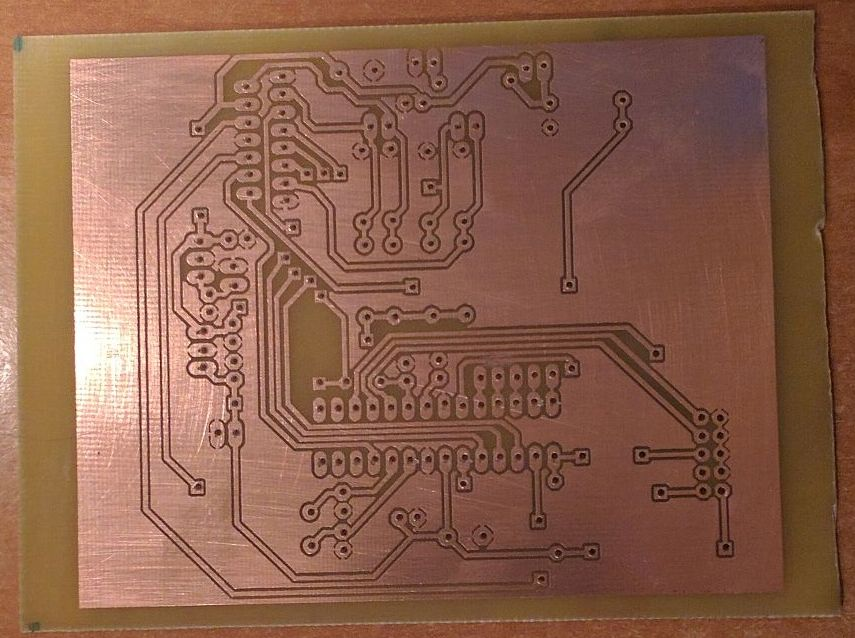
\includegraphics[scale=0.35]{\ImgPath/sterownikdcprzed.jpg}
\end{center}
	\caption{Płytka PCB sterownika silników wytrawiona w roztworze nadsiarczanu sodu [opracowanie własne]}
	\label{schematKomunikacji}
\end{figure}

\begin{figure}[!htbp]
	\begin{center}
\centering
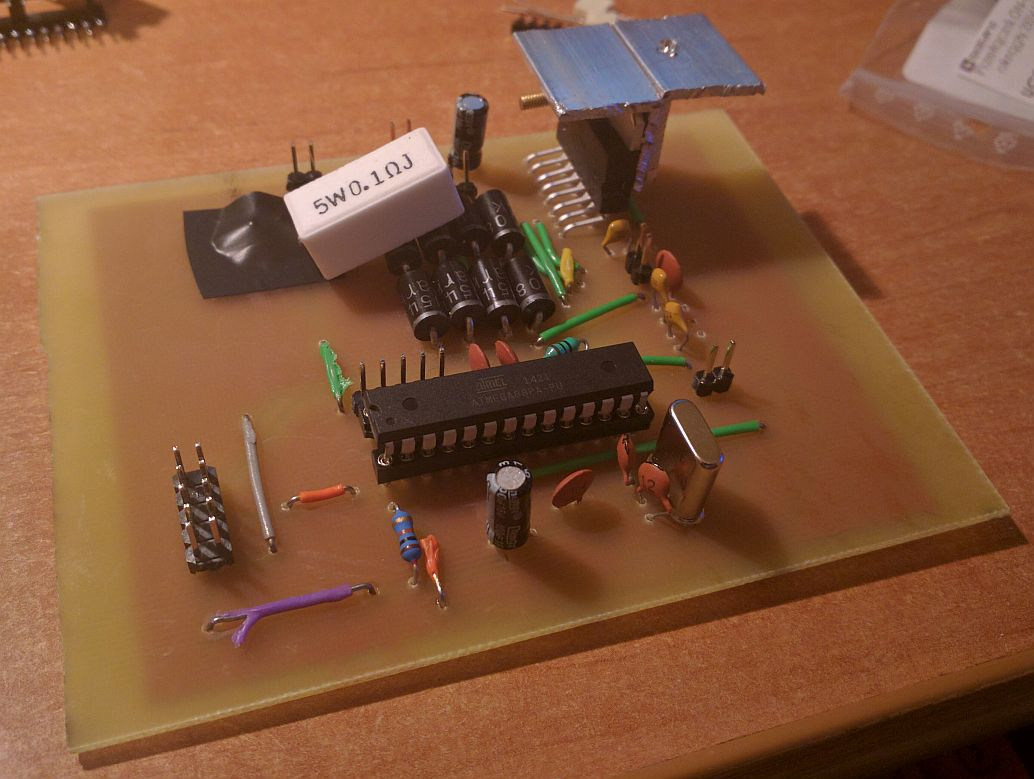
\includegraphics[scale=0.3]{\ImgPath/sterownikdcpo.jpg}
\end{center}
	\caption{Gotowa płytka sterownika silników [opracowanie własne]}
	\label{schematKomunikacji}
\end{figure}

\newpage

  %-----------------
  % Układ regulacji położenia i skanowania pomieszczeń
  %-----------------
\section{Układ regulacji położenia i skanowania pomieszczeń}

Do wykonywania większości obliczeń został wybrany mikrokontroler STM32F103RBTF na płytce NUCLEO. Układ scalony zbiera informacje ze wszystkich czujników robota: enkoderów magnetycznych, akcelerometru, żyroskopu, czujników ultradźwiękowych i modułu WiFi. Następnie wykorzystuje te dane do obliczenia aktualnej prędkości i kierunku obrotów silników, aby utrzymać pion i zeskanować całe pomieszczenie.
Przeprogramowywanie mikrokontrolera jest ułatwione poprzez wbudowany programator na płytce NUCLEO.

\begin{figure}[!htbp]
	\begin{center}
\centering
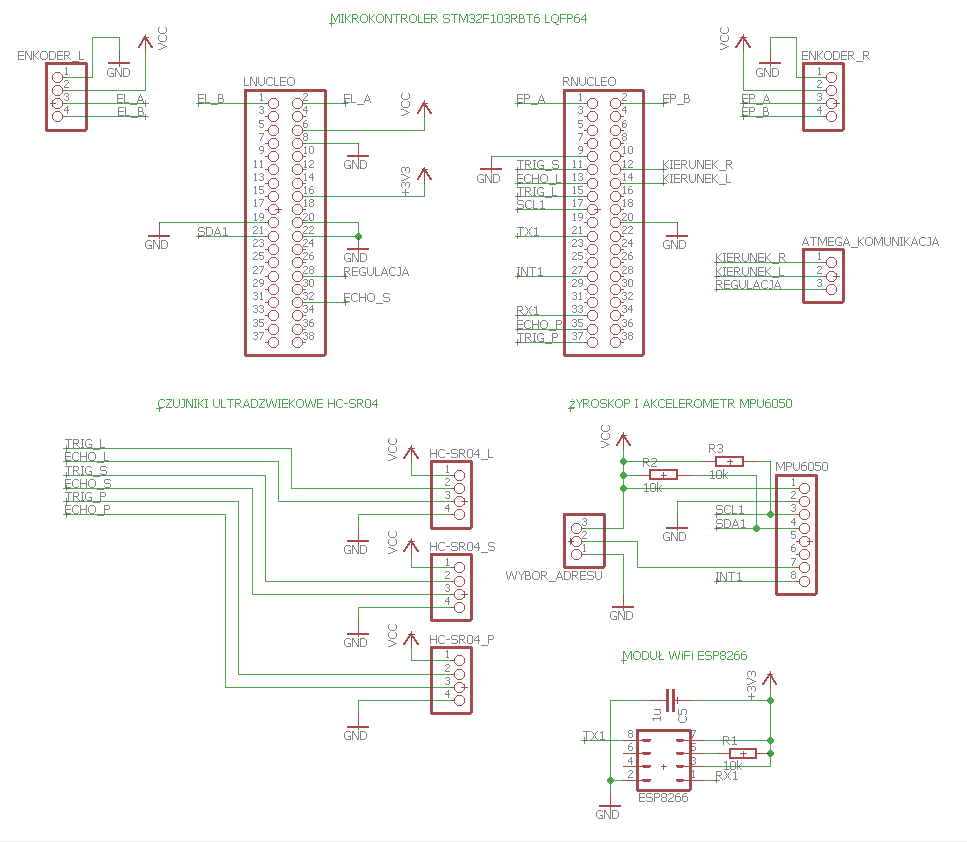
\includegraphics[scale=0.5]{\ImgPath/sterowaniee.PNG}
\end{center}
	\caption{Sposób połączenia elementów elektronicznych układu regulacji położenia i skanowania pomieszczeń wykonany w programie Cadsoft EAGLE [opracowanie własne]}
	\label{schematKomunikacji}
\end{figure}

\newpage

\newpage

\subsection{Mikrokontroler STM32F103RBT6}

Mikrokontroler STM32F103RBT6 32-bitowej architektury ARM na płytce NUCLEO z wyprowadzeniami pinów układu scalonego na złącza goldpin i zintegrowany z programatorem został wybrany ze względu na łatwość montażu i programowania. Architektura używanego mikrokontrolera jest oprarta na rdzeniu Cortex M3, co oznacza dość dużą moc obliczenią przy rozsądnej cenie.\\
Dane techniczne NUCLEO-F103RB:
\begin{itemize}
\item częstotliwość taktowania: 72 MHz,
\item pamięć programu Flash: 128 kB,
\item pamięć SRAM: 20 kB,
\item 2 przetworniki analogowo-cyfrowe: 12-bitowe, 16-kanałowe,
\item 7 timerów,
\item interfejsy: 3 USART, 2 SPI 18 Mbit/s, 2 I2C, USB Full Speed, CAN 2,0B,
\item debugger ST-Link/V2 umieszczony na płytce,
\end{itemize}

\begin{figure}[!htbp]
	\begin{center}
\centering
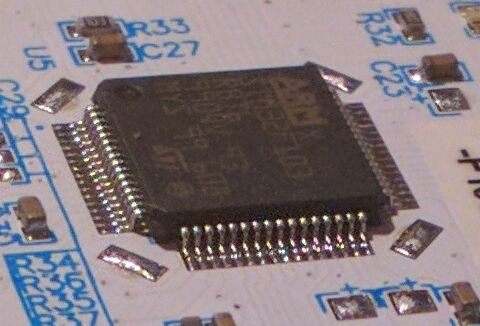
\includegraphics[scale=0.3]{\ImgPath/stm32.jpg}
\end{center}
	\caption{Mikrokontroler STM32F103RBT6 w obudowie LQFP64 [opracowanie własne]}
	\label{schematKomunikacji}
\end{figure}

\begin{figure}[!htbp]
	\begin{center}
\centering
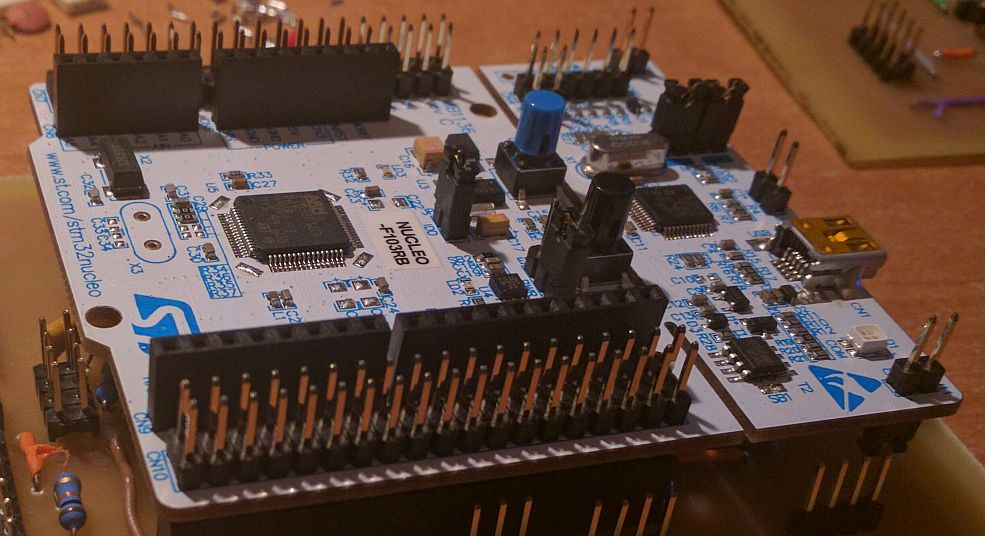
\includegraphics[scale=0.4]{\ImgPath/nucleo.jpg}
\end{center}
	\caption{Płytka NUCLEO-F103RB [opracowanie własne]}
	\label{schematKomunikacji}
\end{figure}

\begin{figure}[!htbp]
	\begin{center}
\centering
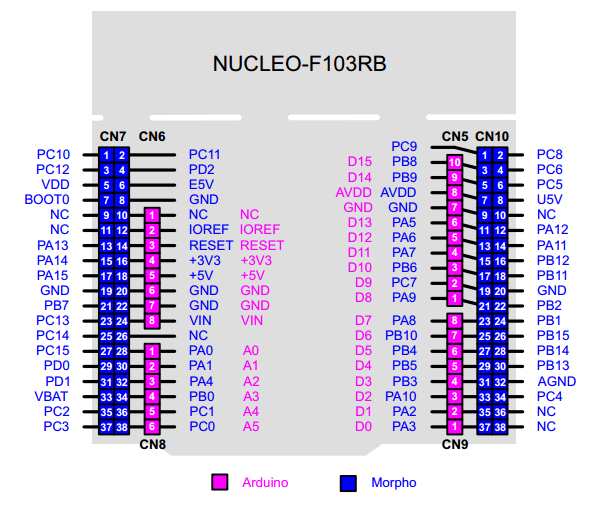
\includegraphics[scale=0.7]{\ImgPath/f103rb.PNG}
\end{center}
	\caption{Wyprowadzenia NUCLEO-F103RB [źródło: bibliografia pkt. 4, strona 30]}
	\label{schematKomunikacji}
\end{figure}

\newpage

Mikrokontroler jest programowany przez złącze Mini USB znajdujące się na płytce. Układ scalony STM32F103RBT6 jest wykorzystywany do zbierania sygnałów ze wszystkich czujników:
\begin{itemize}
\item enkodery magnetyczne - sprzężenie zwrotne w postaci informacji o położeniu kół do układu regulacji położenia w pionie,
\item akcelerometr i żyroskop - sprzężenie zwrotne w postaci informacji o przyspieszeniu kątowym i kącie pochylenia robota do układu regulacji położenia w pionie,
\item czujniki ultradźwiękowe - informacje o położeniu przeszkód na drodze - do układu skanowania pomieszczeń,
\item moduł WiFi - odbieranie informacji o błędach z komputera PC.
\end{itemize}

Zadaniem mikrokontrolera jest przede wszystkim wykorzystać informacje o przebytej drodze i pochyleniu robota do utrzymania pozycji pionowej za pomocą regulatora liniowo-kwadratowego. Sygnały z czujników jako zmienne stanu dodatkowo przechodzą przez filtr Kalmana, co zwiększa ich dokładność. Drugim zadaniem układu scalonego jest zebranie informacji o aktualnej pozycji przeszkód znajdujących się przed robotem i wysłanie ich przez moduł WiFi do sieci lokalnej (co może być odebrane przez dowolne urządzenie obsługujące protokół HTTP). Po każdorazowym wykonaniu tych czynności obliczone wartości prędkości i kierunku obrotu kół są wysyłane do sterownika silników.\\
Połączenie płytki NUCLEO z resztą układu nie wymagało żadnych dodatkowych elementów pasywnych.

\subsection{Żyroskop i akcelerometr - układ MPU6050}

Użyty moduł firmy Invensense zawiera wbudowany cyfrowy żyroskop i akcelerometr. Jego zastosowanie wynika z niskiej ceny i dostatecznych parametrów pracy:
\begin{itemize}
\item napięcie zasilania: 3,3V - 5V,
\item zakresy pracy żyroskopu: 250 dps, 500 dps, 1000 dps, 2500 dps (dps - degrees per second, stopni/sekundę),
\item zakresy pracy akcelerometru: 2g, 4g, 8g, 16g,
\item wymiary: 20mm x 16mm,
\item waga: 0,9 g.
\end{itemize}

\begin{figure}[!htbp]
	\begin{center}
\centering
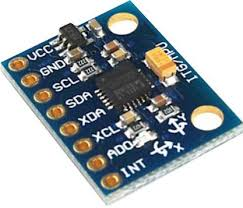
\includegraphics[scale=0.5]{\ImgPath/mpu6050.jpg}
\end{center}
	\caption{Żyroskop i akcelerometr - układ MPU6050 [źródło: https://hobbytronics.com.pk/wp-content/uploads/MPU6050\_1.png]}
	\label{schematKomunikacji}
\end{figure}

Komunikacja z modułem odbywa się za pośrednictwem magistrali szeregowej I2C. Ścieżki SDA i SCL zostały podciągnięte do napięcia zasilania, aby uniknąć stanów nieokreślonych na pinach. 

\begin{figure}[!htbp]
	\begin{center}
\centering
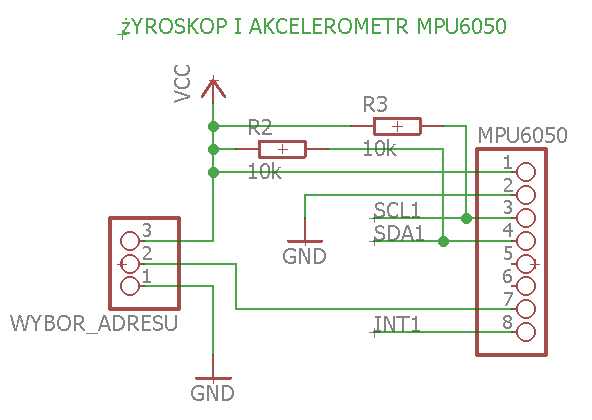
\includegraphics[scale=0.6]{\ImgPath/mpue.PNG}
\end{center}
	\caption{Sposób połączenia czujnika MPU6050 wykonany w programie EAGLE [opracowanie własne]}
	\label{schematKomunikacji}
\end{figure}

\begin{figure}[!htbp]
	\begin{center}
\centering
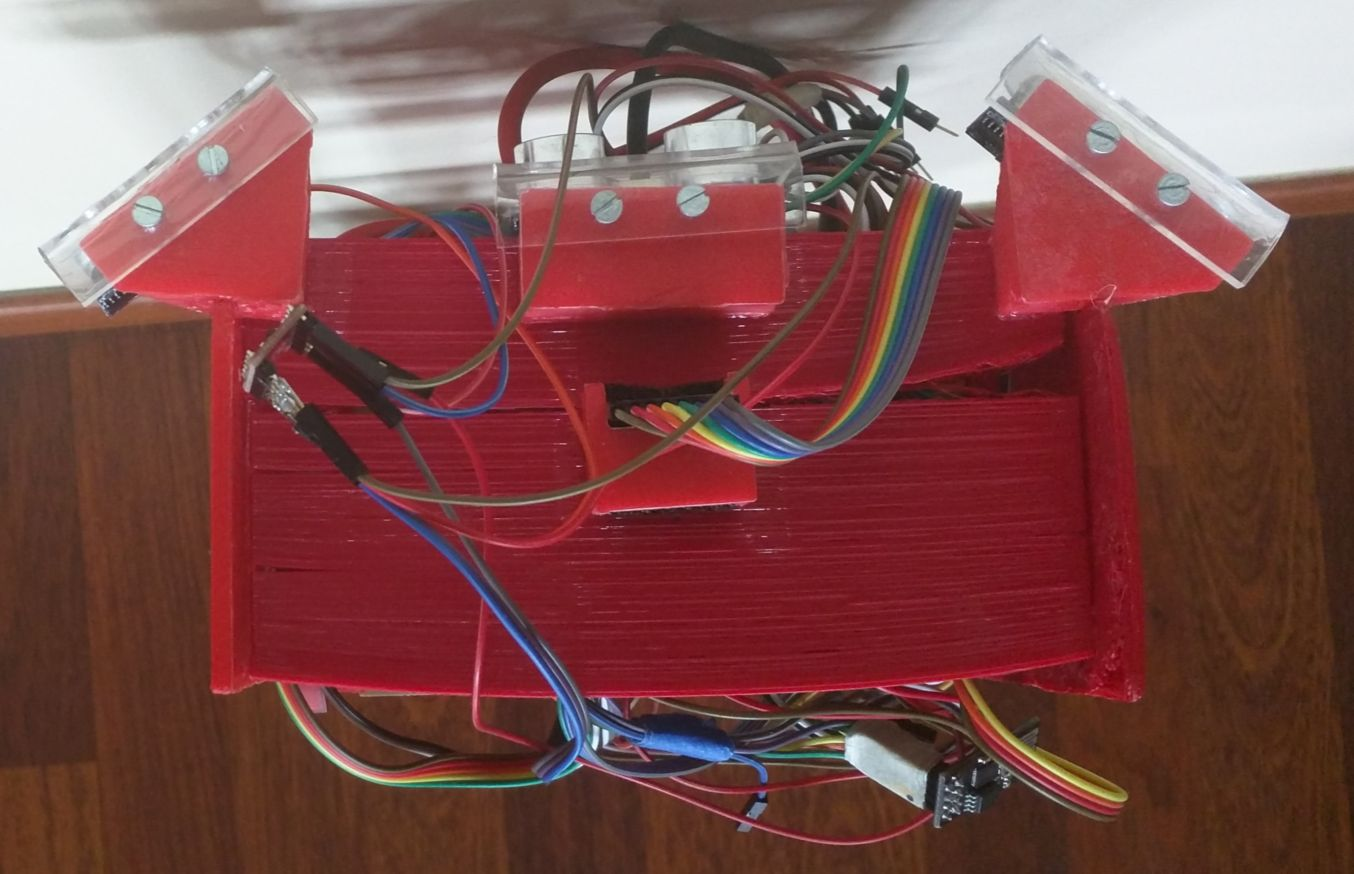
\includegraphics[scale=0.4]{\ImgPath/mpuumieszczenie.jpg}
\end{center}
	\caption{Umiejscowienie czujnika MPU6050 na obudowie robota [opracowanie własne]}
	\label{schematKomunikacji}
\end{figure}

\subsection{Czujniki ultradźwiękowe HC-SR04}

Użyte czujniki HC-SR04 zostały zakupione razem z uchwytami montażowymi. Ich zastosowanie wynika z niskiej ceny i dostatecznych parametrów pracy:
\begin{itemize}
\item napięcie zasilania: 5 V,
\item średni pobór prądu: 15 mA,
\item zakres pomiarowy: od 2 cm do 200 cm,
\item częstotliwość pracy: 40 kHz,
\item wymiary: 45 x 20 x 15 mm.
\end{itemize}

\begin{figure}[!htbp]
	\begin{center}
\centering
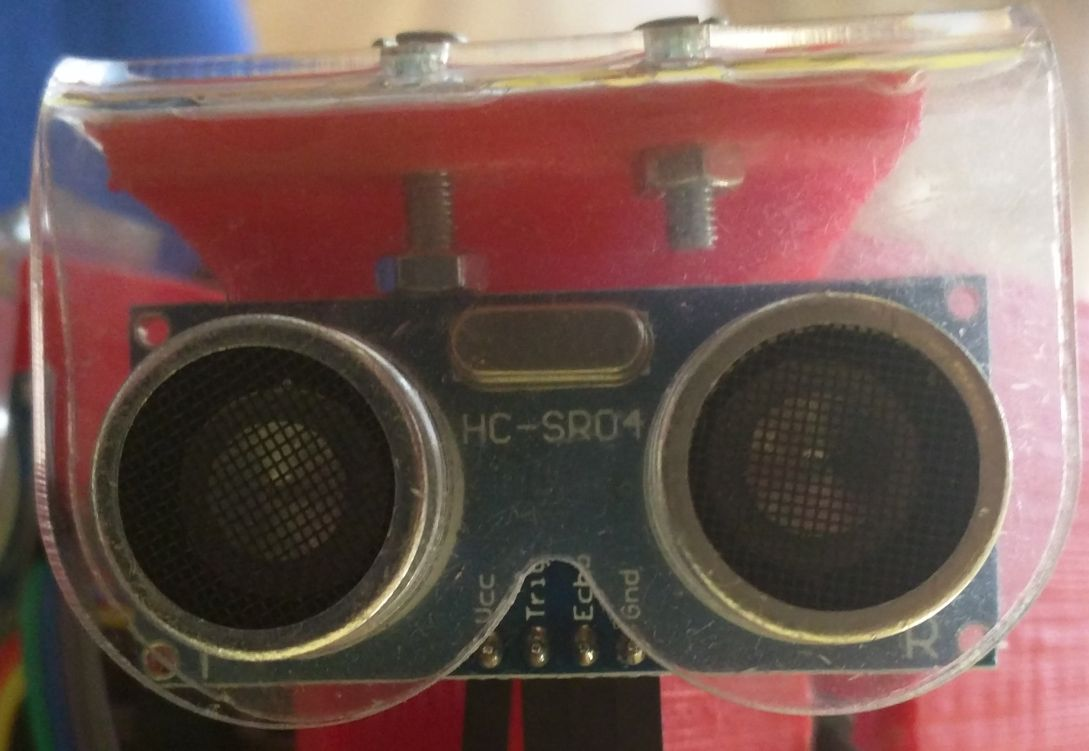
\includegraphics[scale=0.2]{\ImgPath/hcsr04.jpg}
\end{center}
	\caption{Czujniki ultradźwiękowe HC-SR04 [opracowanie własne]}
	\label{schematKomunikacji}
\end{figure}

\newpage

Komunikacja z czujnikami odbywa się za pośrednictwem dwóch pinów: ECHO i TRIG. Wynika to z działania układów. Po podaniu stanu wysokiego na pin TRIG w postaci impulsu trwającego \SI{10}{\micro s} moduł wykonuje pomiar odległości.

Aby rozpocząć pomiar należy podać na pin TRIG impuls napięciowy (stan wysoki 5V) przez \SI{10}{\micro s}. Moduł dokonuje pomiaru odległości przy pomocy fali dźwiękowej o częstotliwości 40 kHz. Na pinie ECHO otrzymywany jest sygnał, w którym odległość od przeszkody jest zależna od czasu trwania stanu wysokiego. Odległość w milimetrach od przeszkody wynosi:\\
$d = 0,17t_{ECHO}$,\\
gdzie:\\
d - odległość mierzona,\\
$t_{echo}$ - czas trwania stanu wysokiego na pinie ECHO.\\
\\
\noindent Wzór jest wyprowadzony z prostej zależności:\\
$d = (t_{echo} × V_{sound})/2$,\\
gdzie:\\
$V_{sound}$ - prędkość rozchodzenia się dźwięku w powietrzu - 340 m/s.

\begin{figure}[!htbp]
	\begin{center}
\centering
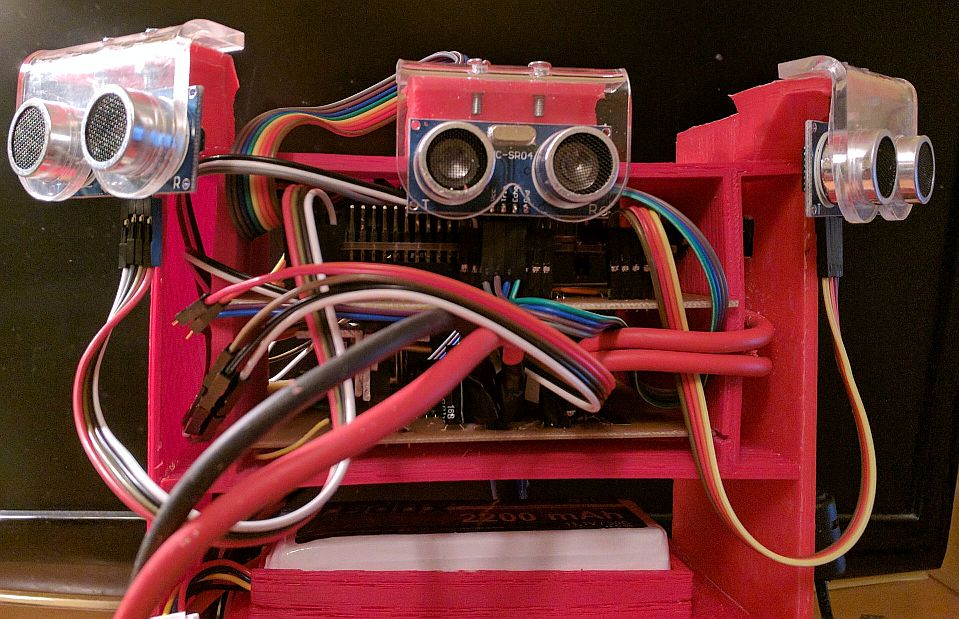
\includegraphics[scale=0.4]{\ImgPath/hcsrumieszczenie.jpg}
\end{center}
	\caption{Umieszczenie czujników HC-SR04 na obudowie robota [opracowanie własne]}
	\label{schematKomunikacji}
\end{figure}

W zestawie znajdują się specjalne uchwyty montażowe, do których zostały zaprojektowane mocowania na szczycie konstrukcji robota. Model w 3D został zaprojektowany w ten sposób, aby czujniki ultradźwiękowe były ustawione: idealnie na wprost jazdy, pod kątem 45\textdegree w prawo i 45\textdegree w lewo. Czujnik najlepiej działa w polu do 30\textdegree od osi prostopadłej do modułu. Stąd od odległości ok. 24 cm od konstrukcji robot będzie miał widoczność w pełnym zakresie 180\textdegree .

\begin{figure}[!htbp]
	\begin{center}
\centering
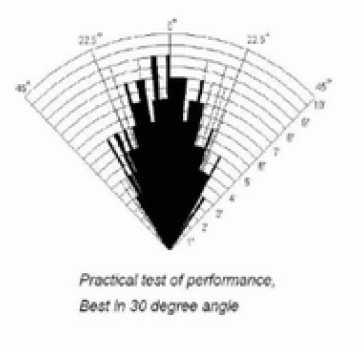
\includegraphics[scale=0.6]{\ImgPath/hcsrzasieg.PNG}
\end{center}
	\caption{Zasięg czujnika HC-SR04 [źródło: bibliografia pkt. 6, strona 4]}
	\label{schematKomunikacji}
\end{figure}

\begin{figure}[!htbp]
	\begin{center}
\centering
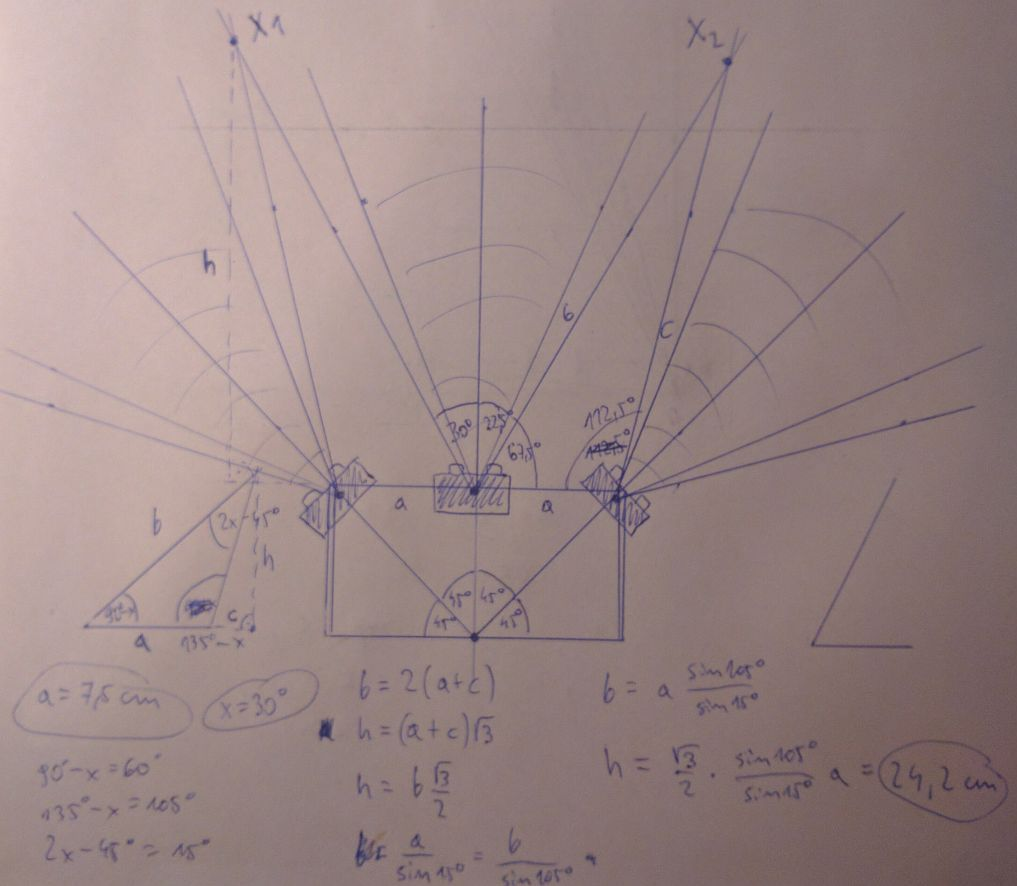
\includegraphics[scale=0.3]{\ImgPath/widocznosc.jpg}
\end{center}
	\caption{Obliczenie obszaru widoczności robota [opracowanie własne]}
	\label{schematKomunikacji}
\end{figure}

\begin{figure}[!htbp]
	\begin{center}
\centering
4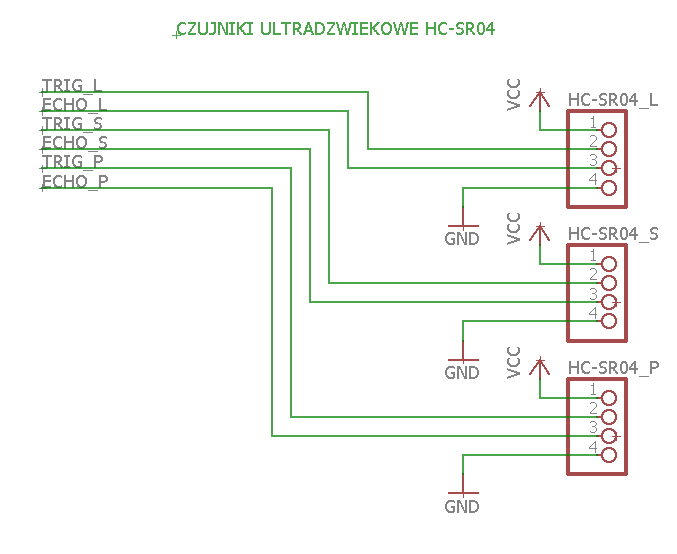
\includegraphics[scale=0.5]{\ImgPath/hcsr04e.PNG}
\end{center}
	\caption{Sposób połączenia czujników HC-SR04 wykonany w programie EAGLE [opracowanie własne]}
	\label{schematKomunikacji}
\end{figure}

\newpage

\subsection{Moduł WiFi ESP-01 8266}

Moduł został wybrany ze względu na niską cenę, powszechne użycie i du żą moc obliczeniową. Dane techniczne:
\begin{itemize}
\item zasilanie: 3,3 V,
\item pamieć Flash: 1 MB,
\item 2 GPIO - wyjścia/wejścia cyfrowe,
\item 1 UART,
\item wbudowana antena PCB,
\item wymiary: 24,8 x 16 mm.
\end{itemize}

\begin{figure}[!htbp]
	\begin{center}
\centering
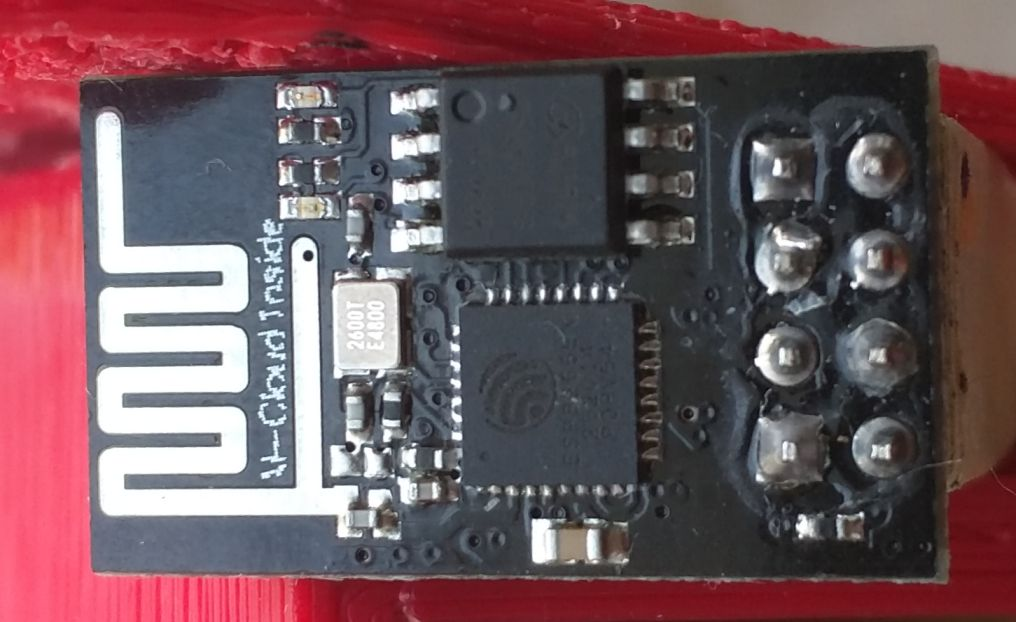
\includegraphics[scale=0.22]{\ImgPath/esp.jpg}
\end{center}
	\caption{Moduł WiFi ESP-01 8266 [opracowanie własne]}
	\label{schematKomunikacji}
\end{figure}

Komunikacja z modułem odbywa się za pośrednictwem interfejsu UART - piny RX i TX. Do prawidłowego działania układu został dołączony kondensator ceramiczny \SI{1}{\micro F} między napięcie zasilania a masę. Piny Reset i CH\_PD zostały podciągnięte do napięcia zasilania modułu, aby dodatkowo ustabilizować pracę urządzenia.

\newpage

\begin{figure}[!htbp]
	\begin{center}
\centering
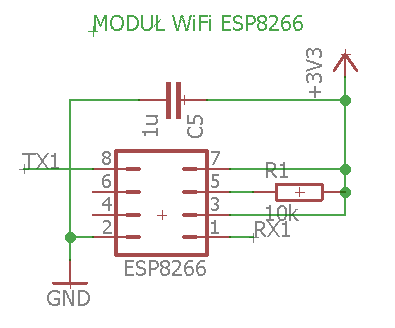
\includegraphics[scale=0.6]{\ImgPath/espe.PNG}
\end{center}
	\caption{Sposób połączenia modułu ESP8266 wykonany w programie EAGLE [opracowanie własne]}
	\label{schematKomunikacji}
\end{figure}

\begin{figure}[!htbp]
	\begin{center}
\centering
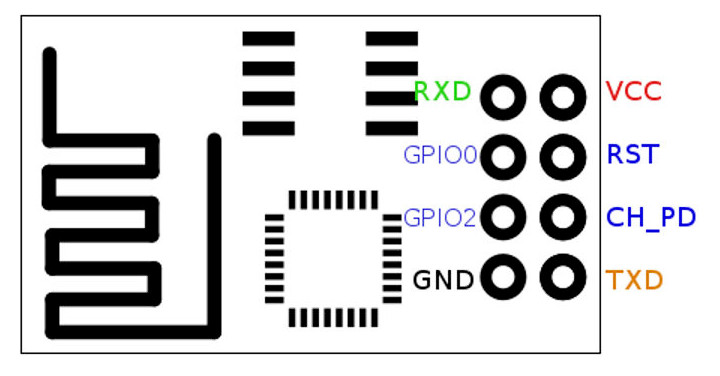
\includegraphics[scale=0.35]{\ImgPath/esp01.jpg}
\end{center}
	\caption{Wyprowadzenia ESP-01 8266 [opracowanie własne]}
	\label{schematKomunikacji}
\end{figure}

Do zaprogramowania modułu należy użyć pinów UART i zewrzeć pino GPIO0 do masy. Z powodu napięcia zasilania ESP8266 3,3 V konieczne jest zastosowanie konwertera napięć, aby podłączyć moduł przez interfejs USB do komputera PC. Dla podwyższonej wygody w tym wypadku został użyty konwerter UART-USB oparty na układzie PL2303, który może pracować na dwóch napięciach 3,3 V i 5 V (wybór napięcia za pomocą zworki).\\
W ESP8266 został wgrany firmware NodeMCU w wersji: nodemcu\_float\_0.9.6-dev\_20150704 za pomocą programu ESP8266Flasher. Nowy firmware umożliwia programowanie modułu za pomocą języka skryptowego Lua, a także w środowisku Arduino, z wykorzystaniem biblioteki esp8266 by ESP8266 Community w wersji 2.3.0-rc2

\newpage

\begin{figure}[!htbp]
	\begin{center}
\centering
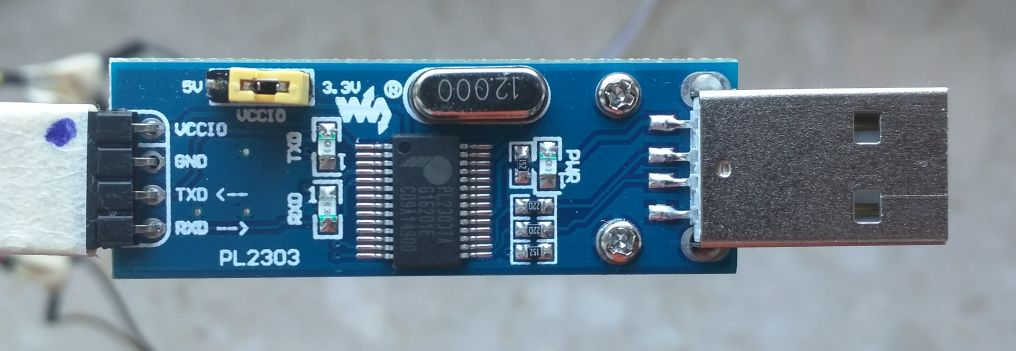
\includegraphics[scale=0.25]{\ImgPath/konwerter.jpg}
\end{center}
	\caption{Konwerter UART-USB oparty na układzie PL2303 [opracowanie własne]}
	\label{schematKomunikacji}
\end{figure}

\subsection{Wykonanie płytki PCB}

Płytka PCB układu regulacji położenia i skanowania pomieszczeń została wykonana w analogiczny sposób jak płytka sterownika silników prądu stałego. Zamiast podstawki precyzyjnej pod mikrokontroler zostały zamontowane żeńskie gniazda goldpin, w których można umieścić płytkę NUCLEO-F103RB.

\begin{figure}[!htbp]
	\begin{center}
\centering
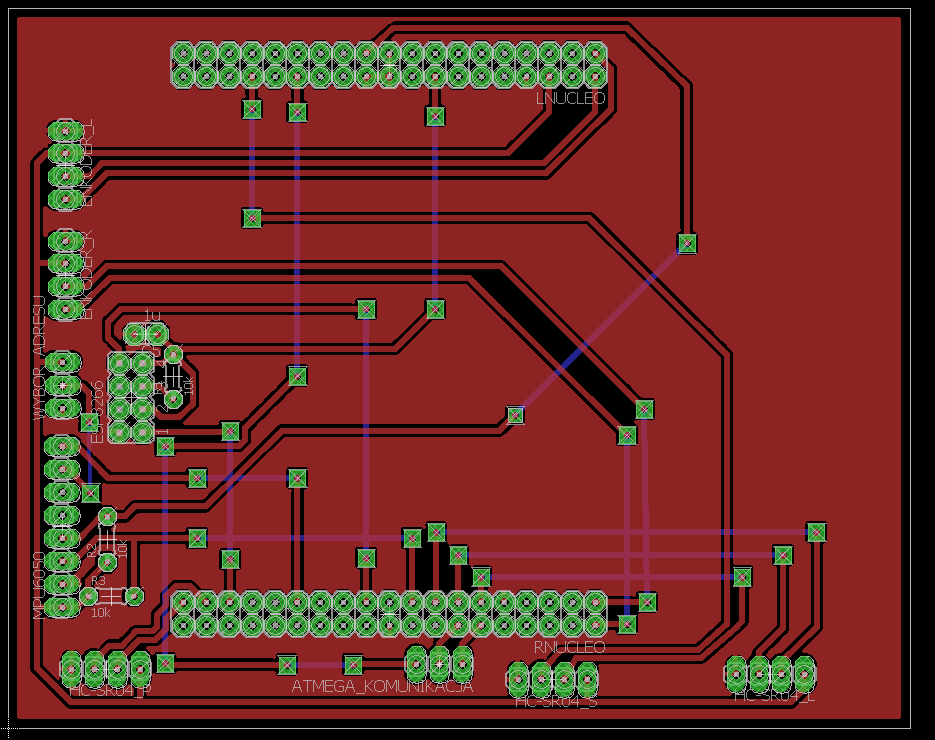
\includegraphics[scale=0.35]{\ImgPath/sterowaniep.PNG}
\end{center}
	\caption{Projekt płytki PCB układu regulacji położenia i skanowania pomieszczeń wykonany w programie Cadsoft EAGLE [opracowanie własne]}
	\label{schematKomunikacji}
\end{figure}

\begin{figure}[!htbp]
	\begin{center}
\centering
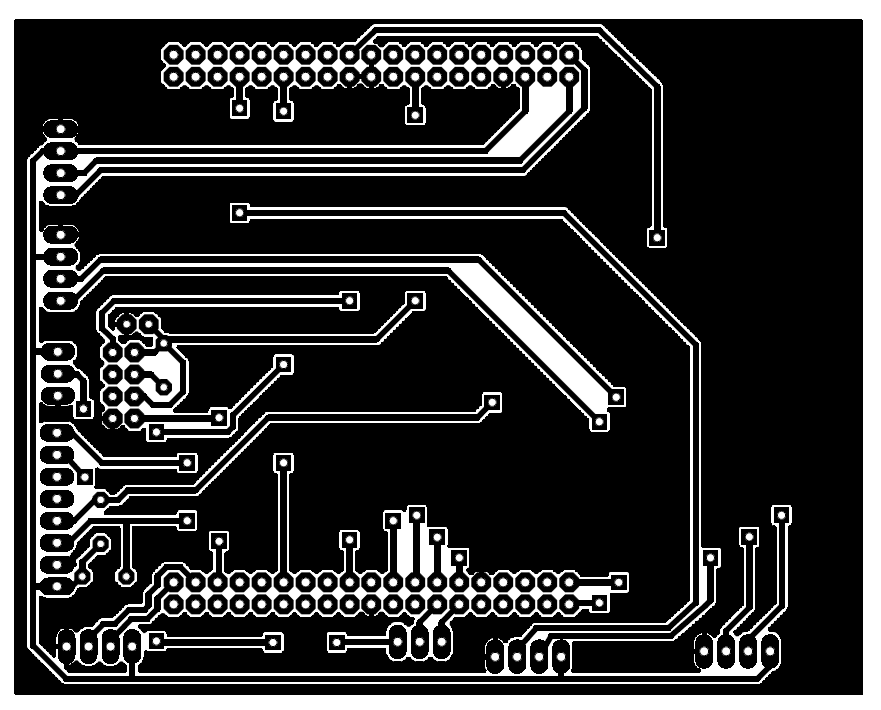
\includegraphics[scale=0.4]{\ImgPath/sterowanied.PNG}
\end{center}
	\caption{Obraz połączeń elementów elektronicznych układu regulacji położenia i skanowania pomieszczeń przygotowany do wydrukowania [opracowanie własne]}
	\label{schematKomunikacji}
\end{figure}

\begin{figure}[!htbp]
	\begin{center}
\centering
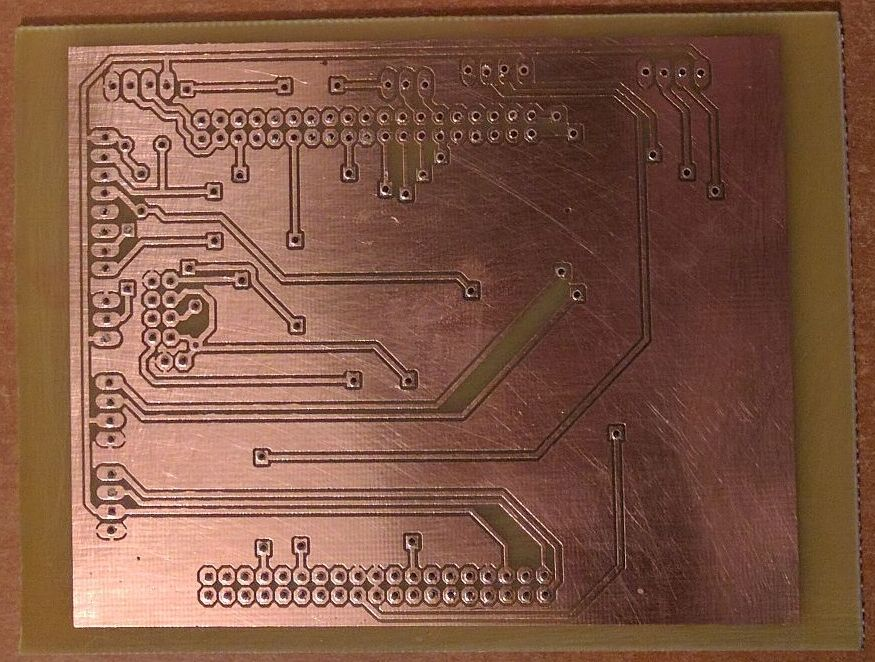
\includegraphics[scale=0.35]{\ImgPath/sterowanie1.jpg}
\end{center}
	\caption{Płytka PCB układu regulacji położenia i skanowania pomieszczeń wytrawiona w roztworze nadsiarczanu sodu [opracowanie własne]}
	\label{schematKomunikacji}
\end{figure}

\begin{figure}[!htbp]
	\begin{center}
\centering
\includegraphics[scale=0.35]{\ImgPath/sterowanie2.jpg}
\end{center}
	\caption{Gotowa płytka układu regulacji położenia i skanowania pomieszczeń bez zamontowanej płytki NUCLEO-F103RB [opracowanie własne]}
	\label{schematKomunikacji}
\end{figure}

\begin{figure}[!htbp]
	\begin{center}
\centering
\includegraphics[scale=0.35]{\ImgPath/sterowanie3.jpg}
\end{center}
	\caption{Gotowa płytka układu regulacji położenia i skanowania pomieszczeń z zamontowaną płytką NUCLEO-F103RB [opracowanie własne]}
	\label{schematKomunikacji}
\end{figure}

\newpage

%-----------------
% Teoria sterowania
%-----------------
\chapter{Teoria Sterowania}

Wykorzystując obliczony model matematyczny układu został zaprojektowany układ sterowania robota w programach Matlab i Simulink. Dobrze zamodelowany układ pozwoli znacznie szybciej dobrać prawidłowe wartości macierzy Q i R w regulatorze liniowo-kwadratowym LQR.

%-----------------
% Wyznaczenie parametrów układu
%-----------------
\section{Wyznaczenie parametrów układu}

Używając gotowych funkcji w Matlabie obliczyłem rzędy macierzy obserwowalności i sterowalności - wynoszą 4. Oznacza to, że skonstruowany układ jest sterowalny i obserwowalny.\\
Układ bez pętli sterowania jest niestabilny - posiada dodatni biegun:\\
\\
$\begin{bmatrix}
0 \\
-11.6894\\
-0.1000\\
11.5017
\end{bmatrix}$
~\\
\\
\noindent Niestabilność układu można zilustrować zasymulowaną odpowiedzią skokową, po zadaniu impulsu dąży do nieskończoności.\\

\newpage

\begin{figure}[!htbp]
	\begin{center}
\centering
\includegraphics[scale=0.4]{\ImgPath/step.jpg}
\end{center}
	\caption{Odpowiedź skokowa układu otwartego [opracowanie własne]}
	\label{schematKomunikacji}
\end{figure}

%-----------------
% Projekt regulatora liniowo-kwadratowego (LQR)
%-----------------
\section{Projekt regulatora liniowo-kwadratowego (LQR)}

Zastosowanie regulatora LQR zapewnia optymalne sterowanie, poprzez zapewnienie dopasowanego wzmocnienia w pętli sprzężenia zwrotnego, ale wymaga dokładnie wyliczonego modelu układu. Założenie projektowe to czas ustalenia odpowiedzi poniżej 1 sekundy.\\
Regulator został zamodelowany w programie Simulink:

\begin{figure}[!htbp]
	\begin{center}
\centering
\includegraphics[scale=0.35]{\ImgPath/lqr.PNG}
\end{center}
	\caption{LQR w programie Simulink [opracowanie własne]}
	\label{schematKomunikacji}
\end{figure}

\newpage

\noindent Macierz wzmocnień K sprzężenia zwrotnego jest obliczana rozwiązując równanie różniczkowe Riccatiego o postaci:\\
\\
$K=R^{-1}B^TP(t)$\\
$\dot{P}(t)=A^TP(t)+P(t)A-P(t)BR^{-1}B^TP(t)+Q$\\

\noindent Gdzie Q i R to macierze wagowe wskaźnika J.
Wartości macierzy Q i R zostały dobrane tak, aby spełnić założenie projektowe:
\begin{itemize}
\item Przemieszczenie robota w przybliżeniu nie większe niż 8 cm: \\$Q_{11} = 1/0.08^2$,
\item Prędkość robota nie większa niż 3 m/s:					$Q_{22} = 1/3^2$,
\item Mały kąt wychylenia wahadła nie większy niż 15\textdegree :	$Q_{33} = 1/15^2$,
\item Prędkość kątowa wychylenia wahadła nie większa niż 30\textdegree/s:\\$Q_{44} = 1/30^2$.
\end{itemize}

Wartości pozostałych elementów macierzy Q przyjąłem jako zerowe – uzyskując w ten sposób macierz symetryczną.
Podobnie dla macierzy R, która ma wymiary 1x1, jest to kwadrat odwrotności największej siły zadziałającej na wahadło czyli ok. 2 N, więc $R = [1/2^2]$.\\

\newpage

\noindent Odpowiedź układu na skok jednostkowy:

\begin{figure}[!htbp]
	\begin{center}
\centering
\includegraphics[scale=0.3]{\ImgPath/lqrstep.PNG}
\end{center}
	\caption{Odpowiedź skokowa układu z LQR w programie Simulink [opracowanie własne]}
	\label{schematKomunikacji}
\end{figure}

\noindent Układ jest stabilny i spełnia założenia projetkowe.\\
\\
\noindent Obliczone Macierze Q i R:\\
\\
$Q=\begin{bmatrix}
       156.2500 & 0 & 0 & 0          \\
       0 & 0.1111 & 0 & 0 \\
       0 & 0 & 0.0044 & 0 \\
       0 & 0 & 0 & 0.0011 
     \end{bmatrix}
$
, $R = [0.2500]$ \\
\\
\\
\noindent Obliczone wzmocnienie LQR:\\

$K=\begin{bmatrix}
       -25.0000 & -12.6331 & 40.5490 & 4.9073
     \end{bmatrix}
$
\\
\\
\noindent Symulacja udowadnia, że teoretycznie jest możliwe ustablizowanie takiego obiektu w pionie.

%-----------------
% Oprogramowanie
%-----------------
\chapter{Oprogramowanie}

Robot został podzielony na kilka modułów, stąd konieczność napisania wielu programów. Każdą część można traktować jako osobny element, co umożliwia wykonywanie testów pojedynczych modułów, bez konieczności podłączania ich do reszty podzespołów. Takie podejście ułatwia wykrycie błędu w całym systemie i zapewnia lepszą diagnostykę.\\
Łączna objętość kodu to 2538 linii.

%-----------------
% Projekt sterowania położenia w pionie (Matlab, Simulink)
%-----------------
\section{Projekt sterowania położenia w pionie (Matlab, Simulink)}

Projekt sterowania został napisany w Matlabie i Simulinku, ponieważ umożliwia to łatwe zaprojektowanie systemu za pomocą bloków oraz testowanie różnych wariantów i parametrów sterowania. \\
Cały program został zapisany w jednym pliku (62 linie). Składowe programu lqr.m:
\begin{itemize}
\item wyliczenia macierzy układu przedstawionych w rozdziale 2.7,
\item obliczenia sterowalności, obserwowalności, biegunów i zasymulowania odpowiedzi skokowej układu, przedstawionych w rozdziale 4.1,
\item obliczenia wzmocnienia LQR i zasymulowania działania na zamodelowanym układzie robota (rozdział 4.2).
\end{itemize}

Do obliczenia sterowalności, obserwowalności, biegunów, wzmocnienia LQR i zasymulowania odpowiedzi skokowej zostały wykorzystane funkcje z biblioteki Matlaba, odpowiednio:
\begin{itemize}
\item ctrb() - sterowalność, zwraca rząd macierzy sterowalności,
\item obser() - obserwowalność, zwraca rząd macierzy obserwowalności,
\item pole() - oblicza bieguny układu,
\item lqr() - oblicza wzmocnienie LQR,
\item step() - symulacja odpowiedzi skokowej układu.
\end{itemize}

%-----------------
% Sterownik silników prądu stałego (C, AVR)
%-----------------
\section{Sterownik silników prądu stałego (C, AVR)}

Program został napisany w środowisku Eclipse Mars, z pluginem AVR, w języku ANSI C. Zegar mikrokontrolera ATMega168PA-PU został ustawiony na 20 MHz, generowany z zewnętrznego rezonatora kwarcowego.\\
Użyte biblioteki:
\begin{itemize}
\item avr/interrupt.h - biblioteka AVR do obsługi przerwań,
\item avr/iom168.h - biblioteka AVR do pinów wejścia/wyjścia dla mikrokontrolera ATmega168,
\item util/delay.h - dla funkcji \_delay\_ms(), która pozwala wprowadzić opóźnienia do programu.
\end{itemize}
Cały program został zapisany w jednym pliku - main.c (157 linii). Składowe programu:
\begin{enumerate}
\item Dyrektywy preprocesora dla użytych pinów i pomocniczych makr.\\
Wpisanie wartości sprzętowych, takich jak, użyte piny w dyrektywach preprocesora umożliwia łatwe przeprowadzenie zmian w programie, w przypadku zmiany któregoś pinu i sprawia, że program staje się bardziej uniwersalny.
\item Deklaracje zmiennych globalnych, słowo kluczowe volatile zapobiega optymalizacji zmiennych przez kompilator, co jest konieczne, w przypadku, gdy zmienne są używane w przerwaniach.
\item Funkcja uint16\_t measure(uint8\_t channel) umożliwiająca pomiar napięcia dla dowolnego pinu ADC mikrokmontrolera (zakres od 0 do 5), za pomocą działań na bitach.
\item Funkcja void hardware\_setup() ustawiająca porty jako wejście/wyjście, konfigurująca ADC, TIMER2, i wyjścia na mostek L298N oraz uruchamia globalną flagę przerwania.\\
Konfiguracja ADC: ADEN - włączenie ADC, ADPSX - prescaler (w tym przypadku ustawiony na 8), REFS0 - ustawienie napięcia odniesienia jako AVCC z dołączonym kondensatorem.\\
Konfiguracja TIMER2: WGM21 - ustawienie trybu CTC, CS21 - prescaler 8, OCR2A - dodatkowy podział częstotliwości przez 200, OCIE2A - ustawienie porównania do rejestru OCR2A\\
sei() - umożliwia używanie przerwań w programie.
\item Funkcja void gather\_data(), która odbiera dane od mikrokontrolera STM32F103RBT6,
\item Funkcja void set\_direction() - ustala kierunek obrotu silników na podstawie danych odebranych funkcją gather\_data(),
\item Procedura obsługi przerwania ISR( TIMER2\_COMPA\_vect ) do obsługi programowego PWM,
\item Główna funkcja programu - int main(void), która zajmuje się ustawianiem odpowiedniego kierunku obrotów silnika i utrzymywania prędkości silników za pomocą sygnału PWM. Konieczne było zastosowanie opóźnienia 2 ms, aby umożliwić stabilną pracę mikrokontrolera.
\end{enumerate}

%-----------------
% Obsługa czujników i sterowanie położenia w pionie (C, StdPeriph)
%-----------------
\section{Obsługa czujników i sterowanie położenia w pionie (C, StdPeriph)}

Główny program sterujący został zaimplementowany w środowisku System Workbench for STM32 opartym na programie Eclipse. Kod został napisany w języku ANSI C. \\
Struktura plików programu:
\begin{itemize}
\item stm32f1xx\_it.h - plik wygenerowany przez środowisko System Workbench do kompilacji projektu (61 linii),
\item syscalls.c - plik wygenerowany przez środowisko System Workbench do minimalnej obsługi zawołań (calls), 204 linie kodu,
\item system\_stm32f10x.c - plik wygenerowany przez środowisko System Workbench, główny kod konfiguracyjny dla mikrokontrolera (częstotliwość taktowania, początkowe ustawienie głównych rejestrów), 379 linii,
\item HAL\_MPU6050.h - plik nagłówkowy biblioteki do obsługi I2C (MIT license Copyright (c) 2012 Harinadha Reddy Chintalapalli) zawierający konfigurację sprzętową - wybór pinów i kanału I2C mikrokontrolera (65 linii),
\item MPU6050.h - plik nagłówkowy biblioteki do obsługi I2C i modułu akcelerometra i żyroskopu MPU6050 (MIT license Copyright (c) 2012 Harinadha Reddy Chintalapalli), zawiera definicję wszystkich rejestrów MPU6050 (428 linii),
\item MPU6050.c - zawiera kod źródłowy dla biblioteki obsługującej 	I2C i moduł MPU6050 (MIT license Copyright (c) 2012 Harinadha Reddy Chintalapalli), obsługuje całą komunikację z MPU6050 i udostępnia funkcję void MPU6050\_GetRawAccelGyro(s16* AccelGyro), która pobiera dane akcelerometru i żyroskopu (465 linii),
\item esp8266.h - plik nagłówkowy do obsługi modułu Wifi ESP8266 (21 linii),
\item esp8266.c - zawiera kod źródłowy części obsługującej moduł WiFi ESP8266, czyli konfigurację UART (53 linie),
\item main.c - plik z programem głównym, zawiera obsługę enkoderów, komunikację z ATmega168PA-PU i MPU6050 oraz sterowanie położenia w pionie (408 linie).
\end{itemize}

Program składa się z 482 linii autorskiego kodu, 644 linii kodu wygenerowanego i 958 linii kodu bibliotecznego, co przekłada się na łączną sumę 2084 linii. Po skompilowaniu program zużywa 35056 bajtów miejsca w pamięci flash mikrokontrolera.

\subsection{Plik HAL\_MPU6050.h}

Komunikacja z modułem MPU6050 została skonfigurowana dla kanału pierwszego magistrali I2C mikrokontrolera STM32F103RBT6. Prędkość transmisji danych to 100 kHz.

\subsection{Plik esp8266.c}

Komunikacja z modułem WiFi ESP8266 została skonfigurowana dla kanału trzeciego USART, baud rate 115200, 8 bitów danych, brak kontroli parzystości i 1 bit stopu. Transmisja jest inicjalizowana przez wysłanie pakietu zawierającego same zera.\\
Zaimplementowanie funkcji int \_\_io\_putchar(int c) pozwala na używanie funkcji formatowanego wydruku danych printf() dla transmisji USART.

\subsection{Plik main.c}

Plik główny programu zbiera dane ze wszystkich czujników co wiąże się z użyciem kilku bibliotek:
\begin{itemize}
\item math.h - biblioteka matematyczna, wykorzystywana do obliczania dwuargumentowego arcusa tangensa,
\item stdbool.h - umożliwia używanie w języku C logicznego typu danych bool,
\item stm32f10x.h - biblioteka środowiska System Workbench for STM32 zawierająca definicje rejestrów i obsługi peryferiów mikrokontrolera STM32F103RBT6,
\item MPU6050.h - biblioteka do obsługi modułu żyroskopu i akcelerometra MPU6050,
\item esp8266.h - biblioteka do modułu WiFi opisana w części 5.3.2.
\end{itemize}
Kod składa się z kilku części:
\begin{enumerate}
\item Deklaracja stałych mechanicznych, matematycznych i elektronicznych:
\begin{itemize}
\item ROTATION\_CONSTANT wyliczone doświadczalnie na podstawie pomiarów odległości z enkoderów, tak aby dać jak najdokładniejszy wynik,
\item WHEEL\_DIAMETER - średnica kół w centymetrach,
\item PI - liczba PI z dokładnościa do 6 miejsc po przecinku,
\item MPU\_CONSTANT - stała, przez która należy podzielić wyniki z MPU6050, aby otrzymać jednostki w układzie SI,
\item ACCELEROMETER\_SENSITIVITY - czułość akcelerometru,
\item GYROSCOPE\_SENSITIVITY - czułość żyroskopu,
\item dt - czas pomiędzy odczytami pomiarów z MPU6050.
\end{itemize}
\item Deklaracje struktur, zmiennych i flag globalnych.
\item Funkcja void delay\_ms(int time) - wprowadza opóźnienia do programu.
\item Funkcja void SysTick\_Handler() - obsługa przerwania od zegara, częstotliwość przerwania zdefiniowana w funkcji atmega\_communication\_init() przy wywołaniu funkcji SysTick\_Config(). W programie funkcja SysTick\_Handler() wykonuje się co 1 ms. Wystawia flagi do obliczeń w pętli głównej programu.
\item Funkcja void global\_variables\_init() - inicjalizuje wszystkie zmienne globalne.
\item Funkcja void set\_pwm(TIM\_OCInitTypeDef channel, int pwm\_nr, int duty\_cycle) - ustawia wypełnienie sprzętowego PWM dla konkretnego pinu,
\item Funkcja float check\_velocity(int encoder\_counter) do dokładnego pomiaru prędkości chwilowej,
\item Funkcja void encoder\_init() - inicjalizuje porty, zegary i przerwania reagujące na zbocza narastające do obsługi enkoderów.
\item Funkcja void atmega\_communication\_init() - uruchamia przerwanie obsługiwane przez funkcję SysTick\_Handler(), inicjalizuje porty, zegary, timery (tryb sprzętowej modulacji szerokości impulsu - PWM) do komunikacji z mikrokontrolerem ATmega168.
\item Funkcja void mpu\_read\_data() - odczytuje surowe dane z modułu MPU6050 i zapisuje je do globalnej struktury measuredData.
\item Funkcje void EXTI9\_5\_IRQHandler() i void EXTI15\_10\_IRQHandler() to procedury obsługi przerwania dla enkoderów, wystawiają flagi do obliczeń w pętli głównej programu.
\item Funkcja void hardware\_setup() - uruchamia wszystkie funkcje konfiguracyjne.
\item Funkcja void export\_data\_wifi() - wysyła dane ze struktury measuredData przez USART do modułu WiFi ESP8266.
\item Funkcja void export\_data\_atmega() - wysyła dane do sterownika silników (mikrokontroler ATmega168) przy pomocy 5 linii, na których jest wysyłany sygnał prostokątny ze zmiennym wypełnieniem. Sygnały są odbierane za pomocą przetwornika analogowo-cyfrowego.
\item Funkcja void ComplementaryFilter(float *pitch) - implementacja filtru komplementarnego do filtrowania odczytu kąta pochylenia robota,
\item Funkcja główna int main(void) - zawiera definicje zmiennych lokalnych (głównie do regulatora PID) i pętlę główną programu, w której odbywa się sprawdzanie poszczególnych flag wystawianych w przerwaniach i wykonywanie kodu przeznaczonego do poszczególnych zadań:
\begin{itemize}
\item flagi l\_cnt\_flag i r\_cnt\_flag - obliczenie pozycji kół i kierunku poruszania się,
\item flaga velocity\_flag - obliczenie drogi i prędkości średniej robota,
\item flaga mpu\_flag - odczyt danych z MPU6050, obliczenie wyjścia regulatora PID i przekształcenie go na wypełnienie sygnału PWM oraz wysłanie wyników do sterownika silników,
\item flaga uart\_flag - wysłanie danych przez USART do modułu ESP8266
\end{itemize}
\end{enumerate}

W kodzie ze szczególną uwagą zadbano o wydajność:
\begin{itemize}
\item zastosowanie sprzętowej modulacji szerokości impulsu (PWM) praktycznie w ogóle nie obciąża mikrokontrolera,
\item stosowanie zmiennych całkowitych ograniczając działania na liczbach zmiennoprzecinkowych,
\item stosowanie zmiennych typu unsigned, co przyspiesza obliczenia dwukrotnie,
\item wystawianie flag w przerwaniach i wykonywanie zadań w pętli głównej programu.
\end{itemize}


%-----------------
% Obsługa modułu WiFi, serwer WWW (C++, HTML, CSS, JS, XML, Arduino)
%-----------------
\section{Obsługa modułu WiFi, serwer WWW (C++, HTML, CSS, JS, XML, Arduino)}

\subsection{Kod C++}

Program został napisany w środowisku Arduino 1.8.2, z wykorzystaniem dodatkowego zestawu płytek esp8266 by ESP8266 Community w wersji 2.3.0-rc2, a dokładnie płytki Generic ESP8266 Module. Cały kod został zapisany w jednym pliku - ajax.ino (325 linii) w języku C++. Wykorzystane biblioteki:
\begin{itemize}
\item ESP8266WiFi.h - umożliwia podłączenie się do konkretnej sieci WiFi,
\item ESP8266WebServer.h - umożliwia utworzenie serwera.
\end{itemize}
Składowe programu:
\begin{enumerate}
\item Deklaracja zmiennych i stałych, a także serwera na porcie 80 - co oznacza konieczność obsługi protokołu HTTP przez klienta.
\item Funkcja void parseData(MeasuredData \&m, char* buffer), która przetwarza wartości odebrane z mikrokontrolera STM32F103RBT6 - umieszcza odpowiednie dane w odpowiednich miejscach struktury MeasuredData.
\item Funkcja void read\_uart() - odczytuje wartości wysłane z mikrokontrolera STM32F103RBT6. Format wysyłanych danych: \\ "x0,x1,x2,x3,x4,x5,x6,x7,x8,x9,x10,;", w przypadku napotkania średnika odczytywanie się zakończy. Następnie jest wywoływana funkcja parseData().
\item Funkcja void buildWebsite() - buduje stronę za pomocą kodu HTML i CSS.
\item Funkcja void buildJavascript() - buduje stronę za pomocą kodu JavaScript.
\item Funkcja void buildXML() - zbiera dane odczytane z interfejsu UART oraz sprawdza czas wykonywania programu i napięcie zasilania modułu za pomocą ADC - w Arduino jest to gotowa funkcja ESP.getVcc(). Zebrane pomiary są zapisywane do dokumentu XML.
\item Funkcja String millis2time() - oblicza czas wykonywania programu za pomocą gotowej funkcji w Arduino - millis() oraz zamienia go na godziny, minuty i sekundy.
\item Funkcje void handleWebsite() i void handleXML() wysyłają dokumenty HTML i XML na server.
\item Funkcja void setup() konfiguruje UART (baud rate 115200) do komunikacji z mikrokontrolerem STM32F103RBT6, podejmuje próbę połączenia z określoną siecią Wifi i wyświetla komunikaty. Najważniejszym komunikatem jest wyświetlenie WiFi.localIP(), czyli dynamicznie przydzielonego adresu IP w sieci lokalnej, dzięki któremu można się połączyć z serwerem. Aby sprawdzić IP konieczne jest podłączenie modułu do jakiegokolwiek terminala (baud rate 115200), zresetowanie ESP8266 i sprawdzenie komunikatu.
\item Funkcja void loop() - główna pętla programu, zajmuje się odczytywaniem danych z UART i obsługą klienta (wyświetleniem zawartości strony).
\end{enumerate}

\subsection{Kod HTML, CSS, JavaScript i XML}

Dokument HTML został napisany w oparciu o języki HTML, CSS, JavaScript. Dane są aktualizowane asynchronicznie przy pomocy dokumentu XML, dzięki technice AJAX - Asynchronous JavaScript and XML. Dzięki takiemu rozwiązaniu w polach wyświetlają się aktualne pomiary bez konieczności odświeżania całej strony. \\
Struktura dokumentu HTML:
\begin{enumerate}
\item Część HEAD napisana w HTML i CSS. Został zastosowany system kodowania Unicode UTF-8 i ustawiony główny styl strony (font, tło).
\item Część SCRIPT zawierająca kod JavaScript.\\
Funkcja createXmlHttpObject() - tworzy nowy obiekt XMLHttpRequest do obsługi zapytań asynchronicznych.\\
Funkcja process() - wykonywana co 200 ms, sprawdza czy obiekt XMLHttpRequest jest otwarty, jeżeli nie, to go otwiera przy pomocy metody PUT i przypisuje funkcję callback handleServerResponse(), gdy obiekt XMLHttpRequest zmieni stan na gotowy.\\
Funkcja handleServerResponse() - otwiera otrzymany dokument XML od obiektu XMLHttpRequest. Przegląda cały dokument i przypisuje odpowiednie wartości do pól w części BODY.
\item część BODY napisana w HTML i CSS. Przy załadowaniu strony jest wywoływana funkcja JavaScript process(), która rozpoczyna proces przetwarzania otrzymywanych dokumentów XML. Dalej jest zapisana struktura strony podzielona na części DIV, w których znajdują się pola $<$A$>$$<$/A$>$ o unikalnych identyfikatorach, pozwalających skryptom JavaScript na lokalizację odpowiednich pól.

Wykorzystywana wersja XML to 1.0. Dokument XML ma prostą strukturę - wszystkie znaczniki znajdują się w głównym znaczniku $<$Donnees$>$$<$/Donnees$>$, a każdy znacznik wewnątrz jednoznacznie identyfikuje pomiar.

\end{enumerate}

%-----------------
% Wnioski 
%-----------------
\chapter{Wnioski}

\TODO

\begin{thebibliography}{99}
\addcontentsline{toc}{chapter}{Bibliografia}
\bibitem{7805}{KEC ,,SEMICONDUCTOR TECHNICAL DATA, KIA7805AP-KIA7824AP BIPOLAR LINEAR INTEGRATED CIRCUIT", 2010.5.19, Revision No: 1.}
\bibitem{LD1117}{STMicroelectronics ,,LD1117 series, Low drop fixed and adjustable positive voltage regulators", December 2006, Rev. 20.}
\bibitem{atmega168}{Atmel Corporation ,,8-bit Atmel Microcontroller with 4/8/16K Bytes In-System Programmable Flash, ATmega48/V, ATmega88/V, ATmega168/V", © 2011 Atmel Corporation, Rev. 2545T–AVR–05/11}
\bibitem{nucleo}{STMicroelectronics ,,UM1724 User manual, STM32 Nucleo-64 board", November 2016, DocID025833 Rev 11}
\bibitem{stm32}{STMicroelectronics ,,RM0008 Reference manual STM32F101xx, STM32F102xx, STM32F103xx, STM32F105xx and
STM32F107xx advanced ARM®-based 32-bit MCUs", November 2015, DocID13902 Rev 16}
\bibitem{hcsr04}{Cytron Technologies ,,Product User’s Manual – HC-SR04 Ultrasonic Sensor", September 2012, V1.0}
\bibitem{segway}{Segway Inc. ,,User Manual Segway Personal Transporter (PT) i2 SE, x2 SE, x2 SE Turf", 2014, 24010-00001 aa}
\bibitem{esp}{Espressif Systems IOT Team ,,ESP8266EX Datasheet", 2015, Version 4.3}
\bibitem{konwerter}{Prolific ,,PL-2303 USB to RS-232 Bridge Controller Product Datasheet", August 2002, Document Revision 1.4}
\bibitem{pololu}{Strona internetowa producenta Pololu ,,9.7:1 Metal Gearmotor 25Dx48L mm MP 12V with 48 CPR Encoder", 27.04.2017, https://www.pololu.com/product/3238}
\bibitem{LD1117}{STMicroelectronics ,,L298 DUAL FULL-BRIDGE DRIVER", January 2000}
\bibitem{nodemcu}{Strona internetowa NodeMcu ,,NodeMcu
Connect Things EASY", 27.04.2017, http://nodemcu.com/index\_en.html}
\bibitem{arduino}{Strona internetowa Arduino ,,Language Reference", 27.04.2017, https://www.arduino.cc/en/Reference/HomePage}
\bibitem{esp8266arduino}{Projekt esp8266/Arduino na Github.com ,,Arduino core for ESP8266 WiFi chip", 27.04.2017, https://github.com/esp8266/Arduino}
\bibitem{harindaha}{Projekt Harinadha/STM32\_MPU6050lib na Github.com ,,MPU6050 I2C Library for STM32f103xx family of microcontrollers", 27.04.2017, https://github.com/Harinadha/STM32\_MPU6050lib}
\bibitem{eclipse}{Strona internetowa Eclipse Foundation, Inc. ,,Eclipse - The Eclipse Foundation open source community website.", 27.04.2017, https://eclipse.org}
\bibitem{eagle}{CadSoft ,,EAGLE - EASILY APPLICABLE GRAPHICAL LAYOUT EDITOR Manual", 2008, Version 5 2nd Edition}
\bibitem{openstm32}{Strona internetowa OpenSTM32 ,,OpenSTM32 CommunityThe STM32 Systems Resource", 27.04.2017, http://www.openstm32.org}
\bibitem{matlab}{Strona internetowa MathWorks ,,MATLAB Documentation", 27.04.2017, https://www.mathworks.com/help/matlab/}
\bibitem{w3}{Strona internetowa w3schools ,,THE WORLD'S LARGEST WEB DEVELOPER SITE", 27.04.2017, https://www.w3schools.com/}


\end{thebibliography}

\zakonczenie  % wklejenie recenzji i opinii

\end{document}
%+++ END +++
